\documentclass[a4paper,10pt]{article}

\usepackage{amsfonts}
\usepackage{amsmath}
% \usepackage{appendix}
\usepackage{graphicx}
\usepackage{hyperref}

\hypersetup{
pdftitle={Derivation of the gyrokinetic equations},
pdfauthor={Gabor Szepesi},
pdfkeywords={gyrokinetics, fully electro-magnetic, guiding-centre, gyrocentre, Lie transform, differential, fundamental one-form},
% bookmarks,
plainpages=false,
pdfborder={0 0 0},
colorlinks=true,
linkcolor=blue,
citecolor=red,
pdfstartview={FitH},
bookmarksopen=false,
unicode
}


%opening
\title{Derivation of the fully electro-magnetic, non-linear, gyrokinetic Vlasov--Maxwell equations in a rotating frame of reference for GKW with Lie transform perturbation method}
\author{G\'abor Szepesi}

\newcommand{\dpt}[1]{\frac{\partial #1}{\partial t}}
\newcommand{\dt}[1]{\frac{\mathrm{d} #1}{\mathrm{d} t}}
\newcommand{\st}[1]{\mathrm{#1}} %subtitle text
\renewcommand{\vec}[1]{\mathbf{#1}}

\graphicspath{{../fig/}}

\begin{document}

\maketitle

% \begin{abstract}
% The new feature of parallel perturbation in the magnetic field has been under development for the gyrokinetic simulation code GKW. Compression of the magnetic field leads to modes which are not present in electrostatic and partially electromagnetic cases, e.g. the compressional Alfv\'en wave, and it is likely to change significantly the growth rates of other modes in the high beta regime. In this work a detailed derivation of the fully electromagnetic gyrokinetic equations in Lagrangian formalism is shown. The transformation of the Lagrangian is performed with the Lie transform perturbation method. A straightforward way of implementation in GKW is discussed.
% \end{abstract}

\tableofcontents

\newpage




%-----------------------------------------------------------------------
\section{Introduction}
In this document the derivation of the gyrokinetic Vlasov--Maxwell system of equations is presented. First, in section \ref{sec:gk_concept}, the main motivation and the basic mathematical concept of the gyrokinetic transformation based on the Lie-transform perturbation method is outlined. A constructive derivation of the gyrokinetic equations is shown in section \ref{sec:gk_derivation}. This calculation is based on the work by Dannert presented in his thesis \cite{dannert}. The main difference is that this derivation includes plasma rotation and is formulated in a co-rotating frame of reference. The gyrokinetic Maxwell-equations are shown in detail, in particular the parallel component of Amp\`ere's law where a minor correction of the equation is suggested. 

The equations derived here are solved by the gyrokinetic code GKW \cite{gkw}. The parallel Amp\`ere's law has recently been implemented in the code and is required for an accurate modelling of high beta discharges. 

%-----------------------------------------------------------------------
\section{Motivation and Basic Mathematical Concept of Gyrokinetics} \label{sec:gk_concept}
Despite the fact that the forces acting on individual particles in a plasma can be analytically expressed, the solution of the equation of motion for every single particle is presently impossible. In order to characterize the macroscopic behaviour of the plasma, such detailed knowledge is not even required. A statistical method, based on describing the evolution of the distribution function of the particles both in real and velocity space, is sufficient. The underlying theory is called the kinetic theory and the equation governing the dynamics of the distribution function is the Vlasov-equation (see any textbook on plasma physics, for example \cite{bellan}):
\begin{equation}
 \dpt{f} + \vec{v} \cdot \frac{\partial f}{\partial \vec{x}} + \vec{a} \cdot \frac{\partial f}{\partial \vec{v}} = 0
 \label{eq:vlasov_basic}
\end{equation}
where $f=f(\vec{x},\vec{v},t)$ is the distribution of the particles in the six-dimensional phase space, $\vec{x}$ is the real spatial coordinate, $\vec{v}$ is the velocity space coordinate, $t$ is time and $\vec{a}$ is the acceleration of particles determined by the force acting on them. Binary interactions between particles can be included in this equation with a collision operator on the right hand side. The study of collisions is in itself a complex area, and for the purpose of this introduction a collisionless case is considered.

Without collisions the particles are accelerated only by electromagnetic forces. The electromagnetic fields are determined by the density and current of the plasma through Maxwell's equations, which are expressed as moments of the distribution function. The acceleration is therefore a non-trivial function of the distribution function and the third term on the left hand side becomes non-linear in $f$. This means that the Vlasov-equation is a complicated integro-differential equation. And the fact that it is six-dimensional (not counting the different species of the plasma), makes its numerical treatment challenging. 

Gyrokinetic theory is basically a method that enables the numerical solution of the Vlasov-equation. The idea is based on the fact that one component of the single particle motion in a magnetized plasma is always a gyration around the magnetic field lines. 
Although gyro-motion leads to fundamental physical phenomena, such as drifts, and therefore strongly influences plasma turbulence, the exact knowledge of where the particles reside on their respective gyro-orbits is not required for estimating macroscopic plasma confinement and transport. The gyro-motion can be averaged out and the orbiting particles replaced by an associated gyro-centre that moves according to the particle drifts. The advantage of gyro-averaging is twofold: first, in an appropriately chosen coordinate system (where the gyro-angle is one of the coordinates), it reduces the dimensionality of the problem from six to five. Second, the gyro-motion typically takes place on a much faster time scale than the turbulent processes of interest. Therefore, once the gyro-averaging has been performed, there is no need to resolve the rapid gyromotion of the particles, and a significantly larger time-step can be applied in the numerical scheme.

In a stationary plasma with uniform magnetic field the projection of the particle orbits onto the plane perpendicular to the magnetic field is a circle. Integrating the particle motion along the gyro-orbit in this case is straightforward since none of the quantities depend on the gyro-phase. 
However, turbulence in plasmas is characterized by small scale and small amplitude fluctuations superimposed on the quasi-stationary equilibrium. These fluctuations vary on the length scale of the Larmor-radius and therefore they reintroduce the gyro-phase dependence to the system. Although a direct averaging over the gyro-angle is still possible, in modern gyrokinetic theory the averaging process is regarded as a phase space transformation. The basic idea is that the six-dimensional phase space manifold is mapped onto itself in a way that the gyro-phase dependence of the fluctuations are asymptotically removed from the equations of motion up to a certain order \cite{brizard}. A rigorous mathematical treatment of the problem is based on the Lie-transform perturbation method \cite{littlejohn_gc}.


%-----------------------------------------------------------------------
\subsection{The Lie-transform Perturbation Method} \label{sec:lie}
The Lie transform perturbation method is a general way of treating small-amplitude perturbations to arbitrary orders with near-identity, continuous mappings of manifolds. The underlying idea is that the points of the manifold are infinitesimally transported along a pre-defined vector field. The vector field can be pictured as a breeze blowing away the points of the manifold, like grains of sand. This defines a mapping $\Phi$ of the manifold $M$ onto itself generated by a vector field $G$: $\Phi: M \to M$. 

%-----------------------------------------------------------------------
\subsubsection{Pull-back, push-forward}
As a result of this mapping not only the points of the manifold are transported, the functions (mapping of the manifold to the real numbers) and curves (mapping of the real numbers to the manifold) change, as well. Figure \ref{fig:pull-back} introduces two important concepts arising from this: the pull-back and push-forward operators. For the sake of generality we define a non-invertible mapping $\Phi$ between two manifolds $M$ and $N$. We assume that there exists a curve on the original manifold $M$ represented by the mapping $\gamma: \mathbb{R} \to M$. One possible definition of a vector space upon a manifold is through finding equivalence classes of curves (for details see \cite{fecko} or any textbook on differential geometry). A vector space upon manifold $M$ will be denoted by $\mathcal{T}^1(M)$ indicating that the vectors lie in the local tangent plane to the manifold. The upper index shows that this is a special, one times contravariant, case of a general $\mathcal{T}_q^p$ tensor space. Note, that a vector space $\mathcal{T}^1(M)$ is not the same as one particular vector field $G$ generating the transform: $G \in \mathcal{T}^1(M)$. The curve $\gamma$ is therefore related to a vector at point $x$ denoted with $\dot{\gamma} \in \mathcal{T}^1(x)$. If we now apply the mapping $\Phi$, the points of curve $\gamma \subset M$ are simply transported to $N$ and thus a curve $\Phi \circ \gamma$ and an associated vector in $\Phi(x)$ naturally arise. The two-step process of moving along the arrows $\gamma$ and $\Phi$ can be substituted by a single mapping from $\mathbb{R}$ directly to $N$. With other words, the curve $\gamma$ and the vector $\dot{\gamma}$ are \emph{pushed forward} from manifold $M$ to $N$ by the mapping $\Phi$. The push-forward operator acting on the vector space is denoted by $\Phi_*$ and the new vector by $\Phi_* \dot{\gamma}$. Note, that this process does not work in the opposite direction: if a curve originally existed on $N$ it could not be pushed forward to $M$ unless $\Phi$ was invertible. However, if a function $\Psi: N \to \mathbb{R}$ is defined on the target manifold $N$ it can be \emph{pulled back} to $M$. Any point on $N$ that is mapped to a certain real value by $\Psi$ has an origin in $M$. Thus, following the two-step process of moving along $\Phi$ and then $\Psi$ can be replaced by a single effective arrow from $M$ to $\mathbb{R}$ $\Psi \circ \Phi$. 

\begin{figure}
 \begin{center}
	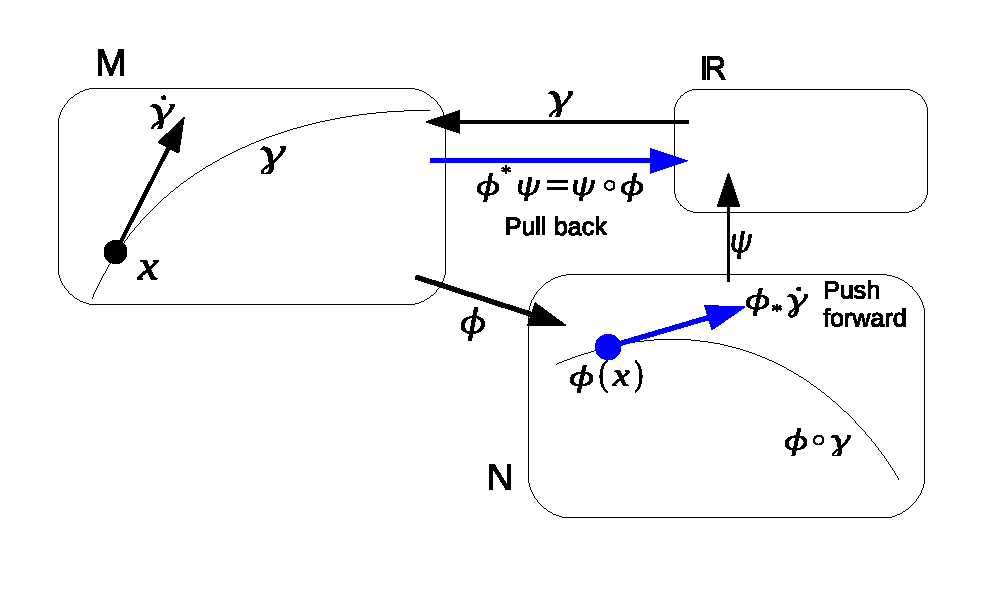
\includegraphics[scale=0.6]{pullback-pushforward-mod.eps}
 \end{center}
 \caption{The pull-back and push-forward operators induced by a general continuous mapping $\Phi$ between two differentiable manifolds $M$ and $N$. Since $\Phi$ is generally not invertible, the existence of a mapping $\mathbb{R} \to M$ induces a mapping $\mathbb{R} \to N$ but not the other way around. Similarly $\Psi: N \to \mathbb{R}$ naturally leads to $\Psi \circ \Phi: M \to \mathbb{R}$.}
 \label{fig:pull-back}
\end{figure}

For our present purpose, the application of Lie-transform method in gyrokinetics, we have to consider an other mathematical object: functions mapping the vectors on a manifold to the real numbers. These can also be thought of as elements of the dual space of the original vector space and denoted as $\mathcal{T}_1(M)$. If we replace $M$ and $N$ on figure \ref{fig:pull-back} with $\mathcal{T}^1(M)$ and $\mathcal{T}^1(N)$, such a mapping will be analogous to $\Psi: N \to \mathbb{R}$ in the previous example. They are therefore pulled back from the vector space upon the target manifold $N$ to that upon $M$. The pull-back operator acting on the dual space $\mathcal{T}_1(N)$ will be denoted by $\Phi^*$. The reason why we have to consider this object is because in the Lagrangian formalism of the gyrokinetic transformation the Lagrangian itself is represented by a differential one-form on the phase space. A complete introduction to differential forms is beyond the scope of this document. We simply state that differential one-forms are elements of the dual vector space upon a manifold. We can therefore conclude, that when the gyrokinetic transformation is applied, the Lagrangian will be transformed by the pull-back operator. 

%-----------------------------------------------------------------------
\subsubsection{Transformation of a one-form}
Let us assume that the infinitesimal transport $\Phi$ on manifold $M$ generated by the vector field $G$ can be expressed as a function of a small parameter $\varepsilon$. If we want to calculate how a general covariant tensor field $A \in \mathcal{T}_q(M)$ changes due to the transport, we have to compare it with its original state \emph{at the same point}. In order to do this, we have to pull the resulting tensor space back to the original manifold. This operation is expressed by the Lie-derivative:
\begin{eqnarray}
	\mathcal{L}_G A &=& \left. \frac{\mathrm{d}}{\mathrm{d} \varepsilon} \right|_0 \Phi^*_{\varepsilon} A  \qquad \Longrightarrow \\
	\Phi^*_{\varepsilon} A &=& A + \varepsilon \mathcal{L}_G A + \mathcal{O}(\varepsilon^2) \qquad \varepsilon \ll 1.
\end{eqnarray}
Note, that the above formula is generally true if $\Phi^*_{\varepsilon}$, and therefore $\Phi$, is differentiable. $\Phi$ is usually assumed to be an exponential function of $\varepsilon$: $\Phi = \st{e}^{\varepsilon G}$ \cite{littlejohn}. This means that the pull-back operator can also be written as an exponential containing the Lie-derivative. If the manifold $M$ is such that Taylor-series converge ($M$ is $C^{\omega}$ class \cite{fecko}) then it can be approximated as
\begin{equation}
	\Phi^*_{\varepsilon} = e^{\varepsilon \mathcal{L}_G} = 1 + \varepsilon \mathcal{L}_G + \frac{\varepsilon^2}{2!} \mathcal{L}_G \mathcal{L}_G + \mathcal{O}(\varepsilon^3).
	\label{eq:pullback_taylor}
\end{equation}

Let $\Gamma \in \mathcal{T}_1(M)$ an arbitrary one-form on $M$. If it was defined on $N$ then it could simply be pulled back to $M$ by $\Phi^*$. However, if we want to evaluate it on the target manifold, we have to apply the inverse of the pull-back operator. The inverse generally exists if $\Phi$ itself is invertible. This, together with the condition on differentiability, requires $\Phi$ to be a diffeomorphism. In this particular case the exponential form of $\Phi$ satisfies this condition and one can write
\begin{equation}
	\left(\Phi^{*}_{\varepsilon}\right)^{-1} = e^{- \varepsilon \mathcal{L}_G} = 1 - \varepsilon \mathcal{L}_G + \frac{\varepsilon^2}{2!} \mathcal{L}_G \mathcal{L}_G + \mathcal{O}(\varepsilon^3)
	\label{eq:pullback_taylor_inv}
\end{equation}
and the one-form on the target manifold as
\begin{equation}
	\bar{\Gamma} = (\Phi_{\varepsilon}^*)^{-1} \Gamma + \mathrm{d}S
	\label{eq:gyro_lagrangian_general}
\end{equation}
where $\bar{\Gamma} \in \mathcal{T}_1(N)$. $\mathrm{d}S$ expresses gauge freedom, that is, we allow for a constant additional term in the one-form. This is related to  the motion being independent up to an additive constant in the Lagrangian. Finally, the Lie-derivative of the one-form in terms of the generating vector field can be calculated using the homotopy formula \cite{littlejohn}:
\begin{equation}
	(\mathcal{L}_G \Gamma)_i = G^j \left( \frac{\partial \Gamma_i}{\partial x^j} - \frac{\partial \Gamma_j}{\partial x^i} \right)
	\label{eq:homotopy}
\end{equation}
where $x^i$ are contravariant coordinates and $G^i$ are the components of the generating vector field. 

%-----------------------------------------------------------------------
\subsubsection{Perturbations} \label{sec:perturbations}
So far we have expressed how an arbitrary one-form changes under an infinitesimal transformation of the manifold. The reason why this is interesting from a practical point of view is perturbations. Perturbations can be modelled by writing the one-form as a sum of contributions of different orders:
\begin{equation}
\Gamma = \Gamma_0 + \varepsilon \Gamma_1 + \varepsilon^2 \Gamma_2 + \dots.
\end{equation}
A series of transformations associated to each of these terms can be introduced and the overall inverse pull-back operator written as
\begin{eqnarray*}
	(\Phi_{\varepsilon}^*)^{-1} &=& \dots e^{-\varepsilon^2 \mathcal{L}_{G_2}} e^{-\varepsilon \mathcal{L}_{G_1}} \\
	&=& 1 - \varepsilon \mathcal{L}_{G_1} + \varepsilon^2 \left( \frac{1}{2} \mathcal{L}_{G_1}^2 - \mathcal{L}_{G_2} \right) + \mathcal{O}(\varepsilon^3)
\end{eqnarray*}
where the second line is obtained by using equation \ref{eq:pullback_taylor_inv} for each of the factors. Finally, substituting to equation \ref{eq:gyro_lagrangian_general} and separating the orders lead to:
\begin{eqnarray*}
	\bar{\Gamma}_0 &=& \Gamma_0 + \mathrm{d}S_0 \\
	\bar{\Gamma}_1 &=& \Gamma_1 - \mathcal{L}_G \Gamma_0 + \mathrm{d}S_1 \\
	\bar{\Gamma}_2 &=& \Gamma_2 - \mathcal{L}_{G_1} \Gamma_1 + \left( \frac{1}{2} \mathcal{L}_{G_1}^2 - \mathcal{L}_{G_2} \right) \Gamma_0 + \mathrm{d}S_2 \\
	&\vdots&
\end{eqnarray*}
This introduction shows how the perturbation method can be applied up to arbitrary orders. In the present work perturbations only up to first order in an appropriate small parameter will be considered. Choosing the zeroth order gauge function $S_0$ to be zero and using the homotopy formula \ref{eq:homotopy}, the first order perturbation can be finally expressed as
\begin{eqnarray}
	\bar{\Gamma}_0 &=& \Gamma_0 \\
	\bar{\Gamma}_{1,i} &=& \Gamma_{1,i} - G_1^{j} \left( \frac{\partial \Gamma_{0,i}}{\partial x^{j}} - \frac{\partial \Gamma_{0,j}}{\partial x^{i}} \right) + \frac{\partial S_1}{\partial x^{i}}. 
	\label{eq:gy_final}
\end{eqnarray}


%-----------------------------------------------------------------------
\subsection{Lagrangian Formalism and Lie-transform in Gyrokinetics} \label{sec:lie_transform_in_gk}
In this work the derivation of the gyrokinetic equations in Lagrangian formalism is presented. In general kinetic theory the Lagrangian is used to derive the equations of motion through the Euler--Lagrange equations (\ref{eq:euler-lagrange}). The time derivatives of the coordinates enter the Vlasov equation which is solved for the distribution function. As mentioned in the introduction of the chapter, the Vlasov-equation is coupled with Maxwell's equations through the dependence of the electro-magnetic fields on the distribution function. An analytical solution of the Vlasov--Maxwell system is rarely possible, typically an iterative method outlined on figure \ref{fig:lagrangian_formalism} is used in numerical schemes. In the first iteration an initial estimate of the electro-magnetic fields is used for the calculations of the distribution function. Then, the fields are updated by solving the Maxwell-equations are solved with the first approximation of the distribution function. The process is continued until convergence is reached. 
\begin{figure}
 \begin{center}
	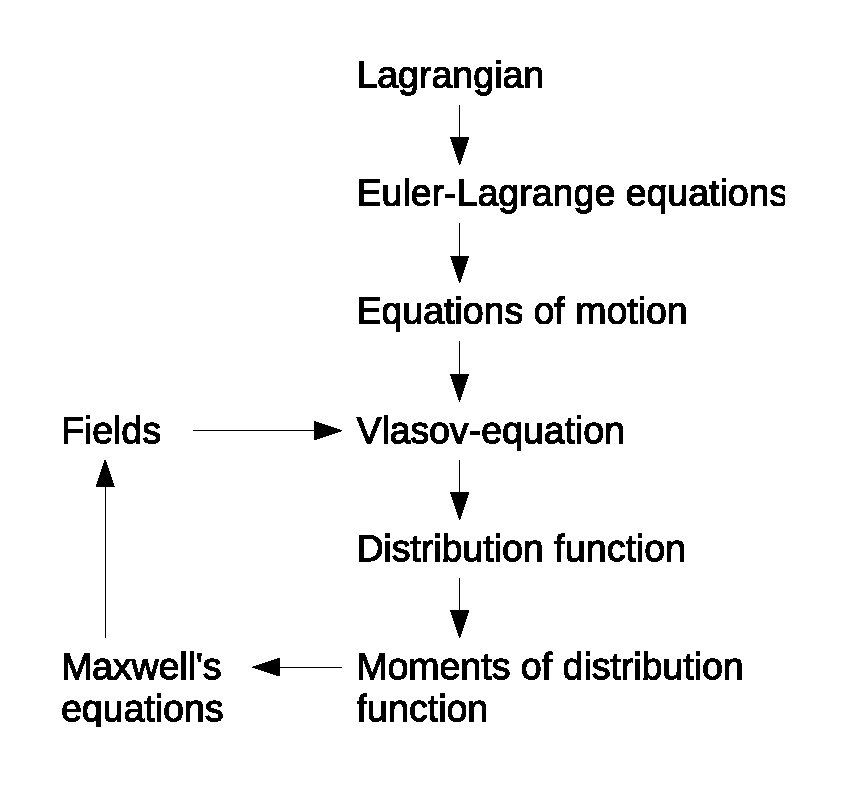
\includegraphics[scale=0.5]{lagrangian-formalism.eps}
 \end{center}
 \caption{Iterative solution of the Vlasov--Maxwell system in Lagrangian formalism.}
 \label{fig:lagrangian_formalism}
\end{figure}

In the previous section (\ref{sec:lie}) it was shown what happens to an arbitrary differential one-form under an infinitesimal transformation of the manifold described by a generating vector field. In gyrokinetics the aim is to find an appropriate transformation of the six-dimensional phase space so that the gyro-angle dependence of the perturbations are asymptotically removed from the Lagrangian. This is now an \emph{inverse} problem: the vector field generating the transport is not specified, its components are derived based on prescribed conditions on the gyrokinetic Lagrangian. 

If the new Lagrangian, the starting point of the graph on figure \ref{fig:lagrangian_formalism} is known, why is it still needed to derive the generating vector field? The gyrokinetic Lagrangian leads to the equations of motion in the transformed coordinates and a Vlasov-equation describing the evolution of the transformed gyrokinetic distribution function. However, the electro-magnetic fields depend on the actual, untransformed positions and velocities of the plasma particles. The transformed distribution function has to be pulled back to the original manifold in order to solve Maxwell's equations. The transformation rule, i.e. the components of the generating vector field, must be derived in order to carry out this pull-back operation. 



%-----------------------------------------------------------------------
\section{Derivation of the Gyrokinetic Equations}  \label{sec:gk_derivation}
The derivation outlined here closely follows the structure of the calculation described by Dannert in his thesis \cite{dannert}. The major difference is that in this work the derivation is performed in presence of finite plasma rotation in a co-rotating frame of reference. 

The derivation of the gyrokinetic equations is carried out through a two-step coordinate transformation method. The first step is a change of coordinates performed in equilibrium without perturbations. The new coordinates are the so called \emph{guiding-centre} coordinates (and the manifold the guiding-centre phase space) which are more suitable to describe the gyrating motion of the charged particles in the stationary magnetic field. The derivation of the guiding-centre Lagrangian is detailed in section \ref{sec:guiding}.

The second step is performed when the perturbations are introduced. It is based on the Lie-transform perturbation method and decouples the gyro-angle dependence of the Lagrangian in the presence of small scale fluctuations. The transformation takes us from the guiding-centre phase space to the so called \emph{gyro-centre} phase space. This process is explained in section \ref{sec:gyro}.

Before proceeding to the derivation of the gyro-kinetic Lagrangian, the ordering assumptions are clarified in section \ref{sec:ordering} and the notation required for the rotating frame of reference is introduced in section \ref{sec:rotation}.

%-----------------------------------------------------------------------
\subsection{Notes on Ordering} \label{sec:ordering}
It has been emphasized in the previous section that the Lie-transform method is applicable for small perturbations. In the general theory this has been expressed by the smallness of the parameter $\varepsilon$ and the linear approximation of the exponential transformation formulae. In gyrokinetic theory the aim is to decouple the effect of small-scale, small amplitude fluctuations of the plasma in the Lagrangian. It is therefore natural to choose either of these properties of the fluctuations as the small parameter in this problem. These statements can be formalized by the usual ordering assumptions applied in gyrokinetic theory \cite{brizard}
\begin{eqnarray}
	\frac{|\mathbf{A}_1|}{|\mathbf{A}_0|} &\sim& \frac{\Phi_1}{\Phi_0} \sim \varepsilon_{\delta} \ll 1 \\ \label{eq:eps_delta}
	\rho \frac{\nabla B_0}{B_0} &\sim& \rho \frac{\nabla E_0}{E_0} \sim \frac{\rho}{L_B} \sim \varepsilon_B  \ll 1\\ \label{eq:eps_B}
	k_{\perp} \rho &\sim& \varepsilon_{\perp} \sim 1 \\ \label{eq:eps_perp}
	\frac{\omega}{\omega_{\st{L}}} &\sim& \varepsilon_{\omega} \ll 1 \label{eq:eps_omega}
\end{eqnarray}
where $\vec{A}$ and $\Phi$ are the vector and scalar potentials, $\vec{B}$ and $\vec{E}$ are the magnetic and electric fields, $\omega$ and $k_{\perp}$ are the typical mode frequency and perpendicular wavenumber, $\rho$ and $\omega_{\st{L}}$ are the Larmor-radius and Larmor-frequency. The equilibrium quantities are denoted with 0 and the fluctuations with 1 subscript. The above equations express that the fluctuations have a much smaller magnitude than the corresponding equilibrium values, their typical time scale is much slower than the Larmor-frequency, their characteristic length scale is of the order of the Larmor-radius and it is typically much shorter than the equilibrium spatial variation scale. The gyrokinetic equation as derived in this document is valid if these ordering assumptions are true. The three different small parameters described here arise for different physical reasons. However, the general practice is to assume that they are of similar order and substitute them with one parameter. In this work the ratio of the reference thermal Larmor-radius and the equilibrium magnetic length scale $\rho_* = \frac{\rho_{\st{ref}}}{L_B} = \frac{m_{\st{ref}} v_{th,ref}}{e B_{\st{ref}}} \sim \varepsilon_B \sim \varepsilon_{\delta} \sim \varepsilon_{\omega}$ is chosen for this purpose, and the equations are derived up to first order in this quantity. 

%-----------------------------------------------------------------------
\subsection{Plasma Rotation} \label{sec:rotation}
Turbulence in a rotating plasma can be conveniently described in a co-rotating
frame of reference. Although a detailed discussion of plasma rotation is outside
the main scope of this document, for the sake of generality the derivation of
the gyrokinetic equations is shown in a reference frame rigidly rotating with
velocity $\vec{u}_0$. The plasma rotation is assumed to be toroidal, the
poloidal component is typically much smaller (the order of the diamagnetic velocity) and neglected here. The reference frame is therefore chosen to rotate in the toroidal direction, and its velocity can be expressed with a constant angular frequency in the form
\begin{equation}
\vec{u}_0 = \vec{\Omega} \times \vec{x} = R^2 \Omega \nabla \varphi
\label{eq:frame_frequency}
\end{equation}
where $\varphi$ is the toroidal angle and $R \nabla \varphi$ is the unit vector in the toroidal direction \cite{peeters_rotation}. 

The rotation of the plasma in the laboratory frame is typically not a rigid body rotation, it is characterized by a radial profile of angular velocity $\hat{\Omega}(\psi)$. The rotating frame is chosen in a way that its angular frequency $\Omega$ matches the plasma rotation at a certain radial point: $\Omega = \hat{\Omega}(\psi_r)$. This method is suitable for local gyrokinetic studies, since in the rotating frame on the surface labelled by $\psi_r$ the plasma rotation vanishes. However, a finite gradient of the rotation profile has to be taken into account. The plasma rotation in the co-rotating frame of reference will be denoted as $\omega_{\varphi}(\psi) = \hat{\Omega}(\psi) - \Omega$. The associated plasma rotation speed along the magnetic field line in the co-rotating frame can be expressed as
\begin{equation}
 u_{\parallel} = \frac{R B_{\st{t}}}{B} \omega_{\varphi}(\psi)
 \label{eq:parallel_rot_speed}
\end{equation}
where $B_{\st{t}}$ is the toroidal component of the magnetic field \cite{peeters_rotation}. 

%-----------------------------------------------------------------------
\subsection{Lagrangian in Guiding-centre Coordinates} \label{sec:guiding}
% In this subsection the Lagrangian, or fundamental one-form, of a plasma particle in guiding-centre coordinates is derived. 
The particle phase space consists of three real and three velocity space components: $(\mathbf{x},\mathbf{v})$. A point in this space describes a particle at a certain position travelling according to a certain velocity vector. The Lagrangian, or fundamental one-form, of a particle with mass $m$ and charge number $Z$ in an electro-magnetic field is written as
\begin{equation}
	\gamma = \gamma_{\nu} \mathrm{d} z^{\nu} = \left( m \mathbf{v} + Z e \mathbf{A}(\mathbf{x}) \right) \cdot \mathrm{d} \mathbf{x} - \left( \frac{1}{2} m v^2 + Z e \Phi(\mathbf{x}) \right) \mathrm{d}t,
\end{equation}
where $\nu$ indexes the six coordinates, and summation over repeated indices is meant \cite{scott_gotit}. $\vec{A}$ and $\Phi$ are the  vector and scalar potentials, respectively. The first term, multiplied by the differential of the spatial coordinates, is called the symplectic part and the second is the Hamiltonian: $H(\mathbf{x},\mathbf{v})$. 
 
In order to write the Lagrangian in a rotating frame of reference, both the velocity coordinates and the fields have to be modified according to the Lorentz-transformation:
\begin{equation}
\vec{v} \to \vec{v} + \vec{u}_0 \qquad \vec{E} \to \vec{E} + \vec{u}_0 \times \vec{B} \qquad \Phi \to \Phi + \vec{A} \cdot \vec{u}_0.
\end{equation}
Following the calculation outlined in \cite{peeters_rotation} the Lagrangian becomes
\begin{equation}
	\gamma = \left( m \mathbf{v} + m \vec{u}_0 + Z e \mathbf{A}(\mathbf{x}) \right) \cdot \mathrm{d} \mathbf{x} - \left( \frac{1}{2} m v^2 + Z e \Phi(\mathbf{x}) - \frac{1}{2} m u_0^2 \right) \mathrm{d}t.
\end{equation}

Let us introduce the guiding-centre phase space with the following coordinate transformation:
\begin{eqnarray}
	\mathbf{X}(\mathbf{x},\mathbf{v}) &=& \mathbf{x} - \mathbf{r} = \mathbf{x} - \rho(\mathbf{x},\vec{v}) \vec{a}(\vec{x},\vec{v}) \label{eq:X}\\
	v_{\parallel}(\mathbf{x},\mathbf{v}) &=& \mathbf{v} \cdot \mathbf{b}(\mathbf{x}) \label{eq:v_par}\\
	\mu(\mathbf{x},\mathbf{v}) &=& \frac{m v_{\st{L}}^2(\mathbf{x})}{2 B(\mathbf{x})} \label{eq:mu}\\
	\theta(\mathbf{x},\mathbf{v}) &=& \cos^{-1} \left( \frac{1}{v_{\st{L}}(\mathbf{x})} (\mathbf{b}(\mathbf{x}) \times \mathbf{v}) \cdot \mathbf{e}_1 \right). \label{eq:theta}
\end{eqnarray}
The new coordinates are the position of the centre of the particle's gyro-orbit, or guiding-centre $\mathbf{X}$, the particle velocity parallel to the equilibrium magnetic field $v_{\parallel}$, the magnetic moment $\mu$ and the gyrophase $\theta$. $\mathbf{b}(\mathbf{x})$ is the unit vector in the direction of the equilibrium magnetic field and $\rho(\mathbf{x},\vec{v}) \vec{a}(\vec{x},\vec{v})$ is the vector pointing from the guiding-centre to the particle's position. Its direction is determined by the unit vector $\vec{a}$ and its length is the Larmor-radius
\begin{equation}
	\rho(\mathbf{x},\vec{v}) = \frac{m v_{\st{L}}(\mathbf{x})}{|Z| e B(\mathbf{x})}
	\label{eq:rho}
\end{equation}
where $v_{\st{L}}$ is the velocity of the gyro-motion, or Larmor-velocity. 
The absolute value of the charge number is needed so the ion and electron Larmor-radii are both positive. The fact that their gyration is in opposite direction is expressed by the vectorial factor $\vec{a}$.
The unit vector $\vec{a}$ can be expressed in a local orthonormal basis as the function of the gyro-angle:
\begin{equation}
	\mathbf{a}(\theta) = \mathbf{e}_1 \cos \theta + \mathbf{e}_2 \sin \theta.
	\label{eq:a}
\end{equation}
The vectors $\mathbf{b}$, $\mathbf{e}_1$ and $\mathbf{e}_2$ form a local righthanded Cartesian coordinate system at the guiding-centre position. 

The transformation of the one-form due to the change of coordinates can be expressed as
\begin{equation}
	\Gamma_{\eta} = \gamma_{\nu} \frac{\mathrm{d} z^{\nu}}{\mathrm{d} Z^{\eta}}
	\label{eq:gc_transform}
\end{equation}
where $\Gamma_{\eta}$ is a component of the guiding-centre fundamental one-form \cite{scott_gotit}. In order to calculate these new components the transformation equations \ref{eq:X}, \ref{eq:v_par}, \ref{eq:mu} and \ref{eq:theta} have to be inverted in order to provide the old coordinates as functions of the new ones: $z(Z)$. It is clear that the direct transformation is uniquely determined if the magnetic field is known at the particle's position. However, when the inverse is taken and particle coordinates are calculated, the particle position can not be explicitly expressed due to the dependence of the Larmor-radius on $\vec{x}$ through the magnetic field. The coordinates are therefore Taylor-expanded in space around the guiding-centre location $\vec{X}$:
\begin{eqnarray*}
	\mathbf{x} &=& \mathbf{X} + \rho(\mathbf{x}) \mathbf{a}(\theta) \\
	\rho(\mathbf{x}) &\approx& \rho(\mathbf{X}) + \left( \frac{\partial \rho(\mathbf{x})}{\partial \mathbf{x}} \right)_{\mathbf{X}} \rho(\mathbf{x}) \mathbf{a}(\theta) + \mathcal{O}((\rho(\mathbf{x}) \mathbf{a}(\theta))^2).
\end{eqnarray*} 
It can be shown that the first order correction in the Taylor-expansion containing $\rho \frac{\partial \rho}{\partial \vec{x}} \sim \rho^2$ leads to second order terms in $\rho_*$. It is thus sufficient to keep only $\rho(\vec{x}) \approx \rho(\vec{X})$ which gives
\begin{equation}
	\vec{x}(\vec{X},\theta) \approx \vec{X} + \rho(\vec{X}) \vec{a}(\theta). \label{eq:x(X)}
\end{equation}
Note that the Larmor radius $\rho$ also depends on the velocity space coordinates $\vec{v}$ in particle phase space, or the magnetic moment $\mu$ in guiding-centre phase space through the formula $\rho(\vec{X},\mu) = \frac{1}{Z e} \sqrt{\frac{2 \mu m}{B(\vec{X})}}$. This dependence will not be explicitly indicated unless greater clarity is called for. 

The particle velocity is the sum of three contributions: the velocity along the magnetic field, the gyration velocity and the drift velocities. It will be shown later that the particle drifts are described by the motion of the guiding centre. Hence the velocity in the guiding-centre frame can be written as
\[\vec{v} = v_{\parallel} \mathbf{b}(\mathbf{x}) + \mathbf{v}_{\st{L}} = v_{\parallel} \mathbf{b}(\mathbf{x}) + \rho(\mathbf{x}) \dot{\mathbf{a}}(\theta)\] 
Applying Taylor expansion again around $\vec{X}$ we obtain
\begin{equation}
	\vec{v}(\vec{X},v_{\parallel},\mu,\theta) \approx v_{\parallel} \left[ \mathbf{b}(\mathbf{X}) + \frac{\partial \mathbf{b}(\mathbf{X})}{\partial \mathbf{X}} \cdot \mathbf{a}(\theta) \rho(\mathbf{X}, \mu) \right] + \rho(\mathbf{X}, \mu) \dot{\mathbf{a}}(\theta)
	\label{eq:v(X)}
\end{equation}

The transformation formula (\ref{eq:gc_transform}) can now be applied to express the fundamental one-form in the new coordinates. The $\vec{X}$ component takes the form
\[ \Gamma_{X^i} = \gamma_{x^j} \frac{\mathrm{d} x^j}{\mathrm{d} X^i} + \underbrace{\gamma_{v^j}}_{0} \frac{\mathrm{d} v^j}{\mathrm{d} X^i} + \gamma_t \underbrace{\frac{\mathrm{d} t}{\mathrm{d} X^i}}_{0}. \]
The required derivative is
\[\frac{\mathrm{d} x^j}{\mathrm{d} X^i} = \delta^j_i + \frac{\mathrm{d} \rho(\mathbf{X})}{\mathrm{d}X^i} a^j(\theta) \]
which substituted into (\ref{eq:gc_transform}) gives
\begin{eqnarray*}
	\Gamma_{X^i} &=& \left( m v_j + m u_{0j} + Z e A_j(\mathbf{x}) \right) \frac{\mathrm{d} x^j}{\mathrm{d} X^i} \\
	&=& \left( m v_{\parallel} b_j(\mathbf{x}) + m \rho(\mathbf{x}) \dot{a}_j(\theta) + m u_{0j} + Z e A_j(\mathbf{x})\right) \left( \delta^j_i + \frac{\mathrm{d} \rho(\mathbf{X})}{\mathrm{d}X^i} a^j(\theta) \right). %\\
\end{eqnarray*}
Expanding the quantities into Taylor-series around $\vec{X}$ and keeping terms up to first order in $\rho$ results
\begin{eqnarray*}
	\Gamma_{X^i} &=& m v_{\parallel} \left[ b_i(\mathbf{X}) + \frac{\partial b_i(\mathbf{X})}{\partial X^k} a^k(\theta) \rho(\mathbf{X}) \right] + m \rho(\mathbf{X}) \dot{a}_i + m u_{0i}\\
	&& + Z e \left[ A_i(\mathbf{X}) + \frac{\partial A_i(\mathbf{X})}{\partial X^k} a^k(\theta) \rho(\mathbf{X}) \right] + (Z e A_j(\mathbf{X}) + m u_{0j}) \frac{\mathrm{d} \rho(\mathbf{X})}{\mathrm{d} X^i} a^j(\theta).
\end{eqnarray*}
Note that $\mathbf{a}$ is perpendicular to both $\mathbf{b}$ and $\dot{\mathbf{a}}$ and the term containing $\rho \frac{\partial \rho}{\partial \vec{X}}$ can be neglected. 

The gyro-averaging operator in guiding-centre phase space is simply an integral over the gyro-phase $\theta$:
\begin{equation}
	\langle \dots \rangle = \frac{1}{2 \pi} \int \limits_0^{2 \pi} \dots \, \mathrm{d} \theta.
\end{equation}
It follows from the definition of the vector $\mathbf{a}$ (equation \ref{eq:a}) that first order terms in $\mathbf{a}$ or $\dot{\mathbf{a}}$ disappear under gyro-averaging. Hence the $\theta$-integral yields
\begin{equation}
	\langle \Gamma_{X^i} \rangle = m v_{\parallel} b_i(\mathbf{X}) + m u_{0i} + Z e A_i(\mathbf{X}).
	\label{eq:gc_X}
\end{equation}

The remaining components are expressed in an analogous way. The parallel velocity component according to equation \ref{eq:gc_transform} becomes
\begin{equation}
	\Gamma_{v_{\parallel}} = \gamma_{\nu} \frac{\mathrm{d}z^{\nu}}{\mathrm{d}v_{\parallel}} = \gamma_{x^i} \underbrace{\frac{\mathrm{d}x^i}{\mathrm{d}v_{\parallel}}}_{0} + \underbrace{\gamma_{v^i}}_{0} \frac{\mathrm{d}v^i}{\mathrm{d}v_{\parallel}} = 0
	\label{eq:gc_vpar}
\end{equation}
meaning that this component remains zero in the guiding-centre approximation. 

The $\mu$-component takes the form
\begin{eqnarray*}
	\Gamma_{\mu} &=& \gamma_{\nu} \frac{\mathrm{d} z^{\nu}}{\mathrm{d} \mu} = \gamma_{x^i} \frac{\mathrm{d}x^i}{\mathrm{d}\mu} = \left( m v_i + m u_{0i} + Z e A_i(\mathbf{x}) \right) \frac{\partial \rho(\mathbf{X},\mu)}{\partial \mu} a^i(\theta) \\
	&=& \left( m v_{\parallel} b_i(\mathbf{x}) + m \rho(\mathbf{x}) \dot{a}_i(\theta) + m u_{0i} + Z e A_i(\mathbf{x}) \right) \frac{\partial \rho(\mathbf{X},\mu)}{\partial \mu} a^i(\theta) \\
	&=& 
	\left[ m u_{0i} + Z e \left( A_i(\mathbf{X}) + \frac{\partial A_i(\mathbf{X})}{\partial X^k} a^k(\theta) \rho(\mathbf{X}, \mu) \right) \right] \frac{\partial \rho(\mathbf{X},\mu)}{\partial \mu} a^i(\theta).
\end{eqnarray*}
Since $\frac{\partial \rho}{\partial \mu} \sim \frac{\rho}{\mu}$, the term containing $\rho \frac{\partial \rho}{\partial \mu}$ leads to second order terms in $\rho_*$ and therefore it can be neglected. Finally, gyro-averaging gives
\begin{eqnarray}
	\langle \Gamma_{\mu} \rangle = 0.
	\label{eq:gc_mu}
\end{eqnarray}

Using relations $\dot{\mathbf{a}}(\theta) = \frac{\partial \mathbf{a}(\theta)}{\partial \theta} \dot{\theta}$ and $\dot{\theta} = \omega_{\st{L}} = \frac{Z e B}{m}$, the gyration velocity can be written as $\rho(\mathbf{X}) \dot{\theta} = \frac{Z}{|Z|} v_{\st{L}}(\mathbf{X})$. Since $\frac{\partial a_i}{\partial \theta} \frac{\partial a^i}{\partial \theta} = 1$ (see equations \ref{eq:a} and \ref{eq:v(X)}) the $\theta$-component becomes
\begin{equation}
	\Gamma_{\theta} = \gamma_{x^i} \frac{\mathrm{d} x^i}{\mathrm{d} \theta} \ \Longrightarrow\ \langle \Gamma_{\theta} \rangle = m \rho(\mathbf{X}) \frac{Z}{|Z|} v_{\st{L}}(\mathbf{X}) = \frac{2 \mu m}{Z e}.
	\label{eq:gc_theta}
\end{equation}

Time is not transformed thus the Hamiltonian part in guiding-centre coordinates remains
\begin{equation}
	\langle \Gamma_t \rangle = -\left( \frac{1}{2} m v_{\parallel}^2 + \mu B(\mathbf{X}) - \frac{1}{2} m u_0^2 + Z e \Phi(\mathbf{X}) \right).
	\label{eq:gc_t}
\end{equation}

Using equations \ref{eq:gc_X}, \ref{eq:gc_vpar}, \ref{eq:gc_mu}, \ref{eq:gc_theta} and \ref{eq:gc_t} describing the components of the fundamental one-form in guiding-centre coordinates we finally obtain
\begin{eqnarray}
	\langle \Gamma \rangle &=& \left( m v_{\parallel} \mathbf{b}(\mathbf{X}) + m \vec{u}_0 + Z e \mathbf{A}(\mathbf{X}) \right) \cdot \mathrm{d}\mathbf{X} + \frac{2 \mu m}{Z e} \mathrm{d} \theta \nonumber \\ 
	&& - \left( \frac{1}{2} m v_{\parallel}^2 + \mu B(\mathbf{X}) - \frac{1}{2} m u_0^2 + Z e \Phi(\mathbf{X}) \right) \mathrm{d}t.
	\label{eq:gc_lagrangian}
\end{eqnarray}
The equations of motion can be derived from equation \ref{eq:gc_lagrangian} with the Euler--Lagrange equations (\ref{eq:euler-lagrange}). The results are the well known drifts of the guiding centre and are not detailed here. However, it is important to note that as a consequence of of the Lagrangian being independent of the gyro-phase $\theta$, the magnetic moment $\mu$ (the associated conjugate coordinate pair of $\theta$) becomes an invariant of the motion: $\dot{\mu}=0$.

%-----------------------------------------------------------------------
\subsection{Lagrangian in Gyro-centre Coordinates} \label{sec:gyro}
In this section the fluctuations are added to the guiding-centre Lagrangian, and a transformation is derived that removes the gyro-phase dependence of the perturbations up to first order in $\rho_*$. The derivation is based on a list of requirements on the new Lagrangian and the transformation is defined in terms of the generating vector field. 

%-----------------------------------------------------------------------
\subsubsection{Perturbed guiding-centre one-form}
Let us introduce small scale perturbations of the electromagnetic fields in the form
\[ \mathbf{A} = \mathbf{A}_0 + \mathbf{A}_1 \qquad \Phi = \Phi_0 + \Phi_1.\]
The equilibrium electric field is typically assumed zero in a stationary plasma, but it has to be kept in case of finite plasma rotation. According to the gyrokinetic ordering the perturbations are first order in the typical small parameters used in gyrokinetics: $\frac{A_1}{A_0} \sim \frac{\Phi_1}{\Phi_0} \sim \rho_*$. The perturbations appear in the particle phase space Lagrangian as
\begin{eqnarray*}
	\gamma &=& \gamma_0 + \gamma_1 \\
	\gamma_0 &=& \left( m \mathbf{v} + m \vec{u}_0 + Z e \mathbf{A}_0(\mathbf{x}) \right) \cdot \mathrm{d} \mathbf{x} - \left( \frac{1}{2} m v^2 - \frac{1}{2} m u_0^2 + Z e \Phi_0(\mathbf{x}) \right) \mathrm{d}t \\
	\gamma_1 &=& Z e \mathbf{A}_1(\mathbf{x}) \cdot \mathrm{d} \mathbf{x} - Z e \Phi_1(\mathbf{x}) \mathrm{d}t.
\end{eqnarray*}
The total Lagrangian has to be transformed first to the guiding-centre and then to gyro-centre phase space. The guiding-centre transformation of the equilibrium part has been completed in section \ref{sec:guiding}. The transformation of the perturbed part of the Lagrangian $\gamma_1$ is analogous to the calculation shown there. An important difference arises from the fact that fluctuating quantities vary on a small length scale and therefore Taylor expansion around the guiding-centre is not advantageous. Their values have to be taken at the particle position which is a function of the gyro-angle in guiding-centre coordinates.

The spatial components of the perturbed guiding-centre one-form are calculated as
\begin{eqnarray*}
	\Gamma_{1,X^i} &=& \gamma_{1,\nu} \frac{\mathrm{d} z^{\nu}}{\mathrm{d} X^i}= Z e A_{1,j}(\mathbf{x}) \left( \delta^j_i + \frac{\mathrm{d} \rho(\mathbf{X})}{\mathrm{d} X^i} a^j(\theta) \right) \\ 
	&=& Z e A_{1,i}(\mathbf{x}) + Z e \frac{\mathrm{d} \rho(\mathbf{X})}{\mathrm{d} X^i} A_{1,j}(\mathbf{x}) a^j(\theta) \\
	&\approx& Z e A_{1,i}(\mathbf{x}).
\end{eqnarray*}
The final approximation can be made because the second term contains $\frac{\partial \rho}{\partial \vec{x}} \vec{A}_1 \sim \rho^2$ and therefore can be neglected. The parallel velocity component remains zero since there are no terms added in the perturbed part
\begin{equation}
	\Gamma_{1,v_{\parallel}} = 0.
\end{equation}
The perturbed $\mu$ component is
\begin{equation}
 \Gamma_{1,\mu} = Z e A_{1,j}(\mathbf{x}) \frac{\rho(\mathbf{X})}{2 \mu} a^j(\theta) = \frac{Z}{|Z|} \frac{1}{v_{\st{L}}(\mathbf{X}, \mu)} \mathbf{A}_1(\mathbf{x}) \cdot \mathbf{a}(\theta),
\end{equation}
the $\theta$ component is
\begin{equation}
	\Gamma_{1,\theta} = Z e A_{1,j}(\mathbf{x}) \rho(\mathbf{X}) \frac{\mathrm{d} a^j(\theta)}{\mathrm{d} \theta} = \frac{Z}{|Z|} \frac{2 \mu}{v_{\st{L}}(\mathbf{X},\mu)} \mathbf{A}_1(\mathbf{x}) \cdot \frac{\mathrm{d} \mathbf{a}(\theta)}{\mathrm{d} \theta},
\end{equation}
and the Hamiltonian becomes
\begin{equation}
	\Gamma_{1,t} = -Z e \Phi_1(\mathbf{x}).
\end{equation}
The perturbed part of the one-form in the guiding-centre phase space can be written as
\begin{equation}
	\Gamma_1 = Z e \mathbf{A}_1(\mathbf{x}) \cdot \mathrm{d} \mathbf{X} + \frac{Z}{|Z|} \frac{\mathbf{A}_1(\mathbf{x}) \cdot \mathbf{a}}{v_{\st{L}}} \mathrm{d} \mu + \frac{Z}{|Z|} \frac{2 \mu}{v_{\st{L}}} \mathbf{A}_1(\mathbf{x}) \cdot \frac{\mathrm{d} \mathbf{a}}{\mathrm{d} \theta} \mathrm{d} \theta - Z e \Phi_1(\mathbf{x}) \mathrm{d}t.
	\label{eq:gc_oneform_pert}
\end{equation}
The complete guiding-centre Lagrangian including perturbations is the sum of equations \ref{eq:gc_lagrangian} and \ref{eq:gc_oneform_pert}. 

%-----------------------------------------------------------------------
\subsubsection{Gyro-centre transformation} \label{sec:gyro_derive}
The aim is now to find a transformation that removes the gyro-angle dependence introduced by the fluctuations from the Lagrangian. Since the perturbations are first order in $\rho_*$, this one-form can be transformed into the gyro-centre phase space according to equation \ref{eq:gy_final}. Note, that the transformation is an inverse pull-back operator, which means that the new Lagrangian in the gyro-centre phase space is expressed in guiding-centre coordinates $(\vec{X},v_{\parallel},\mu,\theta)$ in order to allow the comparison of the two one-forms. However, the transformation does give rise to a new set of gyro-centre coordinates $(\bar{\vec{X}},\bar{v}_{\parallel},\bar{\mu},\bar{\theta)}$ which are not being used in the present section. The gyro-centre Lagrangian will be distinguished from its guiding-centre counterpart with an overbar $\bar{\Gamma}$. 

It is not obvious which vector field to use to generate a transformation that removes the fluctuating quantities from the Lagrangian. Therefore, we do not perform a direct transformation. The vector field is derived based on a simple set of requirements on the gyro-centre Lagrangian suggested by Dannert \cite{dannert}:
\begin{eqnarray*}
	G_{1,t} = 0 &\to& \textrm{no transformation in time} \\
	\bar{\Gamma}_{1,v_{\parallel}} = 0 &\to& \textrm{no $v_{\parallel}$ component} \\
	\bar{\Gamma}_{1,\mu} = 0 &\to& \textrm{no $\mu$ component} \\
	\bar{\Gamma}_{1,\theta} = 0 &\to& \textrm{no change in $\theta$ component} \\
	\bar{\Gamma}_{1,\mathbf{X}} = Z e \langle \mathbf{A}_1(\vec{x}) \rangle &\to& \textrm{the transformation leads to the gyro-average}
\end{eqnarray*}

Let us now apply equation \ref{eq:gy_final} and the requirements above to express the components of the generator vector field that provides the desired Lagrangian. As it was mentioned in section \ref{sec:lie_transform_in_gk}, this can be considered as an inverse problem. The equation for the $\mu$ component is written as
\begin{eqnarray}
	\bar{\Gamma}_{1,\mu} &=& \frac{Z}{|Z|} \frac{\mathbf{A}_1(\mathbf{x}) \cdot \mathbf{a}(\theta)}{v_{\st{L}}(\mathbf{X,\mu})} + G_1^{\theta} \frac{2 m}{Z e} + \frac{\partial S_1}{\partial \mu} = 0 \ \ \Longrightarrow \nonumber \\
	G_1^{\theta} &=& - \frac{Z e}{2 m} \left( \frac{Z}{|Z|} \frac{\mathbf{A}_1(\mathbf{x}) \cdot \mathbf{a}(\theta)}{v_{\st{L}}(\mathbf{X,\mu})} + \frac{\partial S_1}{\partial \mu} \right).
\end{eqnarray}
The equation for the $\theta$ component gives
\begin{eqnarray}
	\bar{\Gamma}_{1,\theta} &=& \frac{Z}{|Z|} \frac{m v_{\st{L}}(\mathbf{X},\mu)}{B_0(\mathbf{X})} \mathbf{A}_1(\mathbf{x}) \cdot \frac{\mathrm{d}\mathbf{a}(\theta)}{\mathrm{d} \theta} - G_1^{\mu} \frac{2 m}{Z e} + \frac{\partial S_1}{\partial \theta} = 0 \ \ \Longrightarrow \nonumber \\
	G_1^{\mu} &=& \frac{Z e}{2 m} \left( \frac{\partial S_1}{\partial \theta} + \frac{Z}{|Z|} \frac{m v_{\st{L}}(\mathbf{X},\mu)}{B_0(\mathbf{X})} \mathbf{A}_1(\mathbf{x}) \cdot \frac{\mathrm{d}\mathbf{a}(\theta)}{\mathrm{d} \theta} \right).
\end{eqnarray}
The $v_{\parallel}$ component leads to
\begin{eqnarray}
	\bar{\Gamma}_{1,v_{\parallel}} &=& G_1^{\mathbf{X}} \cdot m \mathbf{b}_0 + \frac{\partial S_1}{\partial v_{\parallel}} = 0 \ \ \Longrightarrow \nonumber \\
	G_1^{\mathbf{X}} \cdot \mathbf{b}_0 &=& - \frac{1}{m} \frac{\partial S_1}{\partial v_{\parallel}}. \label{eq:G1X}
\end{eqnarray}
The spatial components' transformation can be written as
\begin{eqnarray}
	\bar{\Gamma}_{1,\mathbf{X}} &=& Z e \mathbf{A}_1(\mathbf{x}) + Z e G_1^{\mathbf{X}} \times \underbrace{\nabla \times \left( \mathbf{A}_0(\mathbf{X}) + \frac{m}{Z e} (v_{\parallel} \mathbf{b}_0(\mathbf{X})+\vec{u}_0)\right)}_{\equiv \mathbf{B}_0^{*}(\mathbf{X}) \equiv \nabla \times \mathbf{A}_0^{*}(\mathbf{X})} + \nonumber\\
	&& m G_1^{v_{\parallel}} \mathbf{b}_0(\mathbf{X}) + \nabla S_1 = Z e \langle \mathbf{A}_1(\mathbf{x}) \rangle \ \ \Longrightarrow \nonumber \\
	\noalign{\vskip 0.5 truecm}
	0 &=& Z e \underbrace{(\mathbf{A}_1(\mathbf{x}) - \langle \mathbf{A}_1(\mathbf{x})\rangle)}_{\widetilde{\mathbf{A}}_1(\mathbf{x})} + Z e G_1^{\mathbf{X}} \times \mathbf{B}_0^{*}(\mathbf{X}) - m G_1^{v_{\parallel}} \mathbf{b}_0(\mathbf{X}) + \nabla S_1 \label{eq:gamma_gy_X}
\end{eqnarray}
where the notation $\mathbf{B}_0^{*}(\mathbf{X}) = \nabla \times \left( \mathbf{A}_0(\mathbf{X}) + \frac{m}{Z e} (v_{\parallel} \mathbf{b}_0(\mathbf{X})+\vec{u}_0)\right)$ has been introduced. The scalar and vector potential perturbations are formally separated into a gyro-averaged and an oscillating part:
\begin{eqnarray}
	\mathbf{A}_1 &=& \widetilde{\vec{A}}_1 + \langle \mathbf{A}_1 \rangle \\
	\Phi_1 &=& \widetilde{\Phi}_1 + \langle \Phi_1 \rangle. \label{eq:av_osc_decomp_phi}
\end{eqnarray}
In order to express the required component of the generating vector field, first we take the scalar product of equation \ref{eq:gamma_gy_X} with $B_0^{*}$ to obtain $G_1^{v_{\parallel}}$, then the vector product with $\mathbf{b}_0$ to obtain $G_1^{\mathbf{X}}$.
\begin{eqnarray}
	G_1^{v_{\parallel}} &=& \frac{1}{m B_{0 \parallel}^{*}(\mathbf{X})} \left( Z e \widetilde{\vec{A}}_1(\vec{x}) \cdot \mathbf{B}_0^{*}(\mathbf{X}) + \nabla S_1 \cdot \mathbf{B}_0^{*}(\mathbf{X})\right) \\
	G_1^{\mathbf{X}} &=& -\frac{1}{B_{0 \parallel}^{*}(\mathbf{X})} \left( \widetilde{\vec{A}}_1(\vec{x}) \times \mathbf{b}_0(\mathbf{X}) + \frac{1}{m} \frac{\partial S_1}{\partial v_{\parallel}} \mathbf{B}_0^{*}(\mathbf{X}) + Z e \nabla S_1 \times \mathbf{b}_0(\mathbf{X}) \right)
\end{eqnarray}
where equation \ref{eq:G1X} and $B_{0 \parallel}^{*} = \mathbf{B}_0^{*} \cdot \mathbf{b}_0$ have been used. Finally, the transformation of the Hamiltonian part yields
\begin{eqnarray*}
	\bar{\Gamma}_{1,t} &=& -Z e \Phi_1(\mathbf{x}) + G_1^{\mathbf{X}} \cdot \left( \mu \nabla B_0(\mathbf{X}) + Z e \nabla \Phi_0(\mathbf{X}) \right) + G_1^{v_{\parallel}} m v_{\parallel} + G_1^{\mu} B_0(\mathbf{X}) + \frac{\partial S_1}{\partial t} \\
	&=& -Z e \Phi_1(\mathbf{x}) - \frac{1}{B_{0 \parallel}^{*}} \left( \widetilde{\vec{A}}_1(\vec{x}) \times \mathbf{b}_0(\mathbf{X}) + \frac{1}{m} \frac{\partial S_1}{\partial v_{\parallel}} \mathbf{B}_0^{*}(\mathbf{X}) + Z e \nabla S_1 \times \mathbf{b}_0(\mathbf{X}) \right) \cdot \\
	&& \left( \mu \nabla \mathbf{B}_0(\mathbf{X}) + Z e \nabla \Phi_0(\mathbf{X}) \right) + \frac{v_{\parallel}}{B_{0 \parallel^{*}}} \left( Z e \widetilde{\vec{A}}_1(\vec{x}) \cdot \mathbf{B}_0^{*}(\mathbf{X}) + \nabla S_1 \cdot \mathbf{B}_0^{*}(\mathbf{X})\right) + \\
	&& \frac{Z e}{2 m} \left( \frac{\partial S_1}{\partial \theta} + \frac{Z}{|Z|} \frac{m v_{\st{L}}(\mathbf{X},\mu)}{B_0(\mathbf{X})} \mathbf{A}_1(\mathbf{x}) \cdot \frac{\mathrm{d}\mathbf{a}(\theta)}{\mathrm{d} \theta} \right) B_0(\mathbf{X}) + \frac{\partial S_1}{\partial t}.
\end{eqnarray*}

Let us now take a closer look on the gauge transformation function $S_1$ and its derivatives. According to equations \ref{eq:eps_B}-\ref{eq:eps_perp} the ordering of these derivatives is as follows:
\begin{eqnarray*}
	\partial_t S_1 &\sim& \omega S_1 \sim \varepsilon_{\omega} \omega_{\st{L}} S_1 \sim \rho_* \omega_{\st{L}} S_1 \\
	\nabla_{\parallel} S_1 &\sim& \frac{1}{L_B} S_1 \sim \frac{\rho_*}{\rho} S_1 \\
	\nabla_{\perp} S_1 &\sim& \frac{1}{\rho} S_1 \\
	\partial _{v_{\parallel}} S_1&\sim& \frac{1}{v_{\st{th}}} S_1 \\
	\partial_{\mu} S_1 &\sim& \frac{B_0}{T} S_1 \\
	\partial_{\theta} S_1 &\sim& 1.
\end{eqnarray*}
Note that the characteristic length scale of the perturbations along the magnetic field lines is of order $L_B$ and that the characteristic parallel velocity and Larmor-speed is of order of the thermal velocity. Using the above assumptions and $|\mathbf{B}_0^{*}| = \left| \mathbf{B}_0 + \frac{m v_{\parallel}}{e} \nabla \times \mathbf{b}_0 \right| \sim B_0 + \rho_* B_0$, the ordering of the terms containing $S_1$ in the gyro-centre Hamiltonian can be written as
\begin{eqnarray*}
	\frac{\mathbf{B}_0^{*}}{B_{0 \parallel}^{*}} \frac{1}{m} \frac{\partial S_1}{\partial v_{\parallel}} \cdot (\mu \nabla B_0 + Z e \nabla \Phi_0) &\sim& \rho_* \omega_{\st{L}} \left( 1 + \frac{Z e \Phi_0}{\mu B_0} \right) S_1 \\
	\frac{1}{B_{0 \parallel}^{*}} Z e \nabla S_1 \times \mathbf{b}_0 \cdot (\mu \nabla B_0 + Z e \nabla \Phi_0) &\sim& \rho_* \omega_{\st{L}} \left( 1 + \frac{Z e \Phi_0}{\mu B_0} \right) S_1 \\
	\frac{\mathbf{B}_0^{*}}{B_{0 \parallel}^{*}} \cdot \nabla S_1 v_{\parallel} \sim \frac{v_{\parallel}}{\rho} \varepsilon_B S_1 &\sim& \rho_* \omega_{\st{L}} S_1 \\
	\frac{Z e}{2 m} \frac{\partial S_1}{\partial \theta} B_0 &\sim& \omega_{\st{L}} S_1 \\
	\frac{\partial S_1}{\partial t} &\sim& \rho_* \omega_{\st{L}} S_1
\end{eqnarray*}
Note that $\nabla_{\perp} S_1 \cdot \mathbf{B}_0 = 0$ and $\nabla_{\parallel} S_1 \times \mathbf{b}_0 = 0$. Let us assume that the order of $\frac{Z e \Phi_0}{\mu B_0}$ is no larger than $1$ ($\Phi_0$ is zero in a non-rotating plasma). Terms that are explicitly second order in $\rho_*$ have been neglected. Since $S_1$ is the first order gauge function, $\rho_* S_1$ gives rise to second order terms and therefore can be neglected, as well. The only term that remains is the one containing the $\theta$ derivative of $S_1$. Using the above orderings and applying the decomposition in equation \ref{eq:av_osc_decomp_phi} gives
\begin{eqnarray*}
	\bar{\Gamma}_{1,t} &=& - Z e \left( \widetilde{\Phi}_1(\mathbf{x}) + \langle \Phi_1(\mathbf{x})\rangle \right) - \frac{1}{B_{0 \parallel}^{*}} \widetilde{\vec{A}}_1(\vec{x}) \times \mathbf{b}_0(\mathbf{X}) \cdot \left( \mu \nabla B_0(\mathbf{X}) + Z e \nabla \Phi_0(\mathbf{X})\right) \\ 
	&& + \omega_{\st{L}} \frac{\partial S_1}{\partial \theta} + \frac{v_{\parallel}}{B_{0 \parallel}^{*}} Z e \widetilde{\vec{A}}_1(\vec{x}) \cdot \mathbf{B}_0^{*}(\mathbf{X}) \\
	&& + Z e \left( \langle \mathbf{A}_1(\mathbf{x}) \cdot \vec{v}_{\st{L}}(\mathbf{X},\mu,\theta) \rangle  + \left( \mathbf{A}_1(\mathbf{x}) \cdot \vec{v}_{\st{L}}(\mathbf{X},\mu,\theta) \right)^{\st{osc}} \right)
\end{eqnarray*}
where $\vec{v}_{\st{L}}(\mathbf{X},\mu,\theta) = v_{\st{L}}(\mathbf{X},\mu) \frac{\partial \mathbf{a}(\theta)}{\partial \theta}$. The word ''osc'' in superscript is the same as $\ \widetilde{}$, it denotes the oscillating part of the quantity between the brackets. 

In order to remove the oscillating quantities from the Lagrangian, the term $\omega_{\st{L}} \frac{\partial S_1}{\partial \theta}$ has to cancel them all. This leads to the following equation for $S_1$:
\begin{eqnarray*}
	\frac{\partial S_1}{\partial \theta} &=& \frac{1}{\omega_{\st{L}}} \left( Z e \widetilde{\Phi}_1(\mathbf{x}) + \frac{1}{B_{0 \parallel}^{*}} \widetilde{\vec{A}}_1(\vec{x}) \times \mathbf{b}_0(\mathbf{X}) \cdot \left( \mu \nabla B_0(\mathbf{X}) + Z e \nabla \Phi_0(\mathbf{X})\right) - \right. \\
	&& \left. \frac{v_{\parallel}}{B_{0 \parallel}^{*}} Z e \widetilde{\vec{A}}_1(\vec{x}) \cdot \mathbf{B}_0^{*}(\mathbf{X}) - Z e \left( \mathbf{A}_1(\mathbf{x}) \cdot \vec{v}_{\st{L}}(\mathbf{X},\mu,\theta) \right)^{\st{osc}} \right).
\end{eqnarray*}
As a result, the total gyro-centre Lagrangian becomes
\begin{eqnarray}
	\bar{\Gamma} &=& \bar{\Gamma}_0 + \bar{\Gamma}_1 = \left( m v_{\parallel} \mathbf{b}_0(\mathbf{X}) + m \vec{u}_0 + Z e \mathbf{A}_0(\mathbf{X}) + Z e \langle \mathbf{A}_1(\mathbf{x}) \rangle \right) \cdot \mathrm{d} \mathbf{X} + \frac{2 \mu m}{Z e} \mathrm{d} \theta - \\
	&& \left( \frac{1}{2} m \left( v_{\parallel}^2 - u_0^2 \right) + \mu B_0(\mathbf{X}) + Z e \left( \Phi_0(\vec{X}) + \langle \Phi_1(\mathbf{x}) \rangle \right) - Z e \langle \mathbf{A}_1(\mathbf{x}) \cdot \vec{v}_{\st{L}}(\mathbf{X},\mu,\theta) \rangle \right) \mathrm{d}t. \nonumber
\end{eqnarray} 
The oscillating quantities have thus been systematically removed from the gyro-centre Lagrangian and added to the gauge function. The components of the gyro-centre Lagrangian are again independent of the gyro-phase, and therefore the magnetic moment in the new phase space remains invariant during the particles' motion. 

%-----------------------------------------------------------------------
\subsubsection{Bessel functions}
Gyro-averaging of the fluctuations can be performed by in Fourier-space by separating the quantities' dependence on the gyro-centre position and the Larmor-radius vector:
\begin{eqnarray*}
 \langle \vec{A}_1(\vec{x}) \rangle &=& \langle \vec{A}_1 (\vec{X}+\vec{r}) \rangle = \langle \int \vec{\hat{A}}_1(\vec{k}) \st{e}^{i \vec{k} \cdot (\vec{X}+\vec{r})} \st{d}\vec{k} \rangle \\
 &=& \frac{1}{2 \pi} \int_0^{2 \pi} \int \vec{\hat{A}}_1(\vec{k}) \st{e}^{i \vec{k} \cdot \vec{X}} \st{e}^{i k_{\perp} \rho \cos \theta} \st{d} \vec{k} \st{d} \theta \\
 &=& \int \vec{\hat{A}}_1(\vec{k}) \st{e}^{i \vec{k} \cdot \vec{X}} \underbrace{\frac{1}{2 \pi} \int_0^{2 \pi} \st{e}^{i k_{\perp} \rho \cos \theta} \st{d} \theta}_{J_0(\rho k_{\perp})} \st{d} \vec{k} \\
 &=& \int J_0(\rho k_{\perp}) \vec{\hat{A}}_1(\vec{k}) \st{e}^{i \vec{k} \cdot \vec{X}} \st{d} \vec{k} = J_0(\lambda) \vec{A}_1(\vec{X})
\end{eqnarray*}
where the vector $\vec{r}$ is used in the sense of equation \ref{eq:X}, and the direction of the basis vector $\vec{e}_1$ has been aligned with the wavenumber vector so that $\vec{k}=\vec{e}_1 k_{\perp}$ leading to $\vec{k} \cdot \vec{r} = \rho k_{\perp} \cos \theta$. $J_0$ is a zeroth order Bessel function of the first kind as defined in \cite{a_and_s}. Its argument becomes $\lambda = i \rho \nabla_{\perp}$ during the inverse Fourier transformation. 

Gyro-averaging of the $\langle \vec{A}_1 \cdot \vec{v}_{\st{L}} \rangle$ can be performed in a similar fashion, although through some lengthy algebra. The detailed calculation can be found in Appendix C of \cite{dannert}. The gyro-averaging process eventually gives
\begin{eqnarray*}
	\langle \Phi_1(\mathbf{x})\rangle &=& J_0(\lambda) \Phi_1(\mathbf{X}) \\
	\langle \mathbf{A}_1(\mathbf{x})\rangle &=& J_0(\lambda) \mathbf{A}_1(\mathbf{X}) \\
	Z e \langle \mathbf{A}_1(\mathbf{x}) \cdot \vec{v}_{\st{L}}(\mathbf{X},\mu,\theta) \rangle &=& - \hat{J}_1(\lambda) \mu B_{1 \parallel}(\mathbf{X})
\end{eqnarray*}
where $\hat{J}_1(z) = \frac{2}{z} J_1(z)$ is a modified first order Bessel function of the first kind.
Substituting the above expressions into the gyro-centre Lagrangian gives
\begin{eqnarray}
	\bar{\Gamma} &=& \left( m v_{\parallel} \mathbf{b}_0(\mathbf{X}) + Z e \mathbf{A}_0(\mathbf{X}) + m \vec{u}_0 + Z e J_0(\lambda) \mathbf{A}_1(\mathbf{X}) \right) \cdot \mathrm{d} \mathbf{X} + \frac{2 \mu m}{Z e} \mathrm{d} \theta - \nonumber\\
	&& \left( \frac{1}{2} m \left( v_{\parallel}^2 - u_0^2 \right) + Z e \left( \Phi_0(\vec{X}) + J_0(\lambda) \Phi_1(\mathbf{X}) \right) + \mu \left( B_0(\mathbf{X}) + \hat{J}_1(\lambda) B_{1 \parallel}(\mathbf{X}) \right) \right) \mathrm{d}t \nonumber \\
	&=& \left( Z e \mathbf{A}_0^{*}(\mathbf{X}) + Z e \bar{\mathbf{A}}_1(\mathbf{X}) \right) \cdot \mathrm{d} \mathbf{X} + \frac{2 \mu m}{Z e} \mathrm{d} \theta - \nonumber\\
	&& \left( \frac{1}{2} m \left( v_{\parallel}^2 - u_0^2 \right) + Z e \left( \Phi_0(\vec{X}) + \bar{\Phi}_1(\mathbf{X}) \right) + \mu \left( B_0(\mathbf{X}) + \bar{B}_{1 \parallel}(\mathbf{X}) \right) \right) \mathrm{d}t
	\label{eq:gyro_oneform}
\end{eqnarray} 
where we used $\mathbf{A}_0^{*} = \mathbf{A}_0 + \frac{m }{Z e} (v_{\parallel} \mathbf{b}_0 + \vec{u}_0 )$ again and introduced the shorter notations $J_0(\lambda) \Phi_1 = \bar{\Phi}_1$, $J_0(\lambda) \mathbf{A}_1 = \bar{\mathbf{A}}_1$ and $\hat{J}_1(\lambda) B_{1 \parallel} = \bar{B}_{1 \parallel}$.


%-----------------------------------------------------------------------
\subsection{Gyrokinetic Vlasov-equation} \label{sec:vlasov}
The time evolution of the distribution function in the phase space is described by the Vlasov equation. In particle phase space without collisions it can be written as
\[ \frac{\partial f}{\partial t} + \dot{\mathbf{x}} \cdot \frac{\partial f}{\partial \mathbf{x}} + \dot{\mathbf{v}} \cdot \frac{\partial f}{\partial \mathbf{v}} = 0.\]
Since in gyro-centre phase space the gyro-phase is an ignorable coordinate and the total time derivative of the gyro-centre magnetic moment is zero (see equation (\ref{eq:gyro_eqs_motion})), the Vlasov equation takes the form
\begin{equation}
	\frac{\partial f_{\st{gy}}}{\partial t} + \dot{\mathbf{X}} \cdot \frac{\partial f_{\st{gy}}}{\partial \mathbf{X}} + \dot{v}_{\parallel} \frac{\partial f_{\st{gy}}}{\partial v_{\parallel}} = 0
	\label{eq:gyro_vlasov}
\end{equation}
where $f_{\st{gy}}$ is the distribution function of they gyro-centres instead of the particles. In the remainder of this section the ''gy'' underscript will be dropped for simplicity and $f$ will denote the gyro-centre distribution function unless otherwise stated. 

Two important modifications have to be performed on equation \ref{eq:gyro_vlasov}: first, the terms $\dot{\mathbf{X}}$ and $\dot{v}_{\parallel}$ have to be expressed from the gyro-centre Lagrangian through of the Euler--Lagrange equations, and second, the total distribution function $f$ will be decomposed into a sum of an equilibrium and a perturbation part: $f = F + \delta f$ where $\frac{\delta f}{F} \sim \varepsilon_{\delta}$. The latter step is the so called delta-f approximation. 

%-----------------------------------------------------------------------
\subsubsection{The Euler--Lagrange equations}
According to Scott \cite{scott_gotit} the Euler--Lagrange equations can be written as
\begin{equation}
	\left( \frac{\partial \gamma_j}{\partial z^i} - \frac{\partial \gamma_i}{\partial z^j} \right) \frac{\mathrm{d} z^j}{\mathrm{d} t} = \frac{\partial H}{\partial z^i} + \frac{\partial \gamma_i}{\partial t}.
	\label{eq:euler-lagrange}
\end{equation}
After substituting equation \ref{eq:gyro_oneform} the equations of motion are directly obtained as
\begin{eqnarray}
 	&& m \dot{v}_{\parallel} \mathbf{b}_0 - Z e \dot{\mathbf{X}} \times \mathbf{B}_0^{*} - Z e \dot{\mathbf{X}} \times \left( \nabla \times \bar{\mathbf{A}}_1 \right) =  \label{eq:gyro_eqs_motion} \\
	&& \hspace{2cm} \underbrace{- Z e \nabla \left( \Phi_0 + \bar{\Phi}_1 \right) - Z e \frac{\mathrm{d}}{\mathrm{d}t} \bar{\mathbf{A}}_1}_{Z e \bar{\mathbf{E}}} - \mu \nabla \left( B_0 + \bar{B}_{1 \parallel}\right) + \frac{1}{2}m \nabla u_0^2 \nonumber \\
	&& v_{\parallel} = \mathbf{b}_0 \cdot \dot{\mathbf{X}} \qquad \dot{\mu} = 0 \qquad \dot{\theta} = \omega_{\st{L}} - \frac{Z e}{m} \frac{\partial}{\partial \mu} \left( Z e \bar{\mathbf{A}}_1 \cdot \dot{\mathbf{X}} - Z e \bar{\Phi}_1 - \mu \bar{B}_{1 \parallel} \right) \nonumber
\end{eqnarray}
where the relation $\left(\nabla \mathbf{A} - (\nabla \mathbf{A})^T \right) \cdot \dot{\mathbf{X}} = \dot{\mathbf{X}} \times (\nabla \times \mathbf{A})$ has been applied. Using equation \ref{eq:frame_frequency} the last term in the first equation of \ref{eq:gyro_eqs_motion} can be rewritten as $\frac{1}{2}m \nabla u_0^2 = m R \Omega^2 \nabla R$. 

By introducing the notation $\nabla \times \bar{\mathbf{A}}_1 = \bar{\mathbf{B}}_1$ and taking the cross product with $\mathbf{b}_0$ the time evolution of the gyro-centre position $\dot{\mathbf{X}}$ can be expressed as
\begin{eqnarray}
	\dot{\mathbf{X}} &=& \mathbf{b}_0 v_{\parallel} + \frac{m v_{\parallel}^2}{Z e B_0} \left( \nabla \times \mathbf{b}_0 \right)_{\perp} + \frac{\bar{\mathbf{B}}_{1 \perp}}{B_0} v_{\parallel} - \frac{1}{B_0} \bar{\mathbf{E}} \times \mathbf{b}_0 + \nonumber \\
	&& \frac{\mu}{Z e B_0} \nabla \left( B_0 + \bar{B}_{1 \parallel} \right) \times \mathbf{b}_0 + \frac{2 m v_{\parallel}}{Z e B_0} \vec{\Omega}_{\perp} - \frac{m R \Omega^2}{Z e B_0} \nabla R \times \vec{b}_0 \nonumber \\
	&=& \mathbf{b}_0 v_{\parallel} + \underbrace{\mathbf{v}_{\bar{\vec{B}}_{1 \perp}} + \mathbf{v}_{\bar{\vec{E}} \times \vec{B}_0} + \mathbf{v}_{\nabla \bar{B}_{1\parallel}}}_{\vec{v}_{\chi}} + \underbrace{\mathbf{v}_{C} + \mathbf{v}_{\nabla \vec{B}_0} + \vec{v}_{\st{co}} + \vec{v}_{\st{cf}}}_{\mathbf{v}_{\st{D}}}.
	\label{eq:gyro_Xdot}
\end{eqnarray}
To obtain equation \ref{eq:gyro_Xdot} the Taylor expansion
\[\frac{1}{B_{0 \parallel}^{*} + \bar{B}_{1 \parallel}} = \frac{1}{B_0} \left( 1 - \frac{m}{Z e B_0} \mathbf{b}_0 \cdot \nabla \times ( v_{\parallel} \mathbf{b}_0 + \vec{u}_0) - \frac{\bar{B}_{1 \parallel}}{B_0}  + O(\rho^2) \right)\]
has been used and the terms were kept up to first order in $\rho_*$. 

The subsequent terms in the first two lines of equation \ref{eq:gyro_Xdot} denote streaming along the equilibrium magnetic field ($\mathbf{b}_0 v_{\parallel}$), curvature drift ($\mathbf{v}_C$), streaming along the perpendicular perturbed magnetic field ($\mathbf{v}_{\bar{\vec{B}}_{1\perp}}$), $E \times B$ drift in the total electric field ($\mathbf{v}_{\bar{\vec{E}} \times \vec{B}_0}$), and grad-$B$ drifts in the gradients of the equilibrium as well as the parallel perturbed magnetic fields ($\mathbf{v}_{\nabla \bar{B}_{1 \parallel}}$ and $\mathbf{v}_{\nabla \vec{B}_0}$), the Coriolis ($\vec{v}_{\st{co}}$) and centrifugal ($\vec{v}_{\st{cf}}$) drifts, respectively.

Note that the motion along the parallel component of the perturbed magnetic field is missing in equation \ref{eq:gyro_Xdot}, it would only appear in higher orders. The perpendicular component of the perturbed vector potential $\bar{\mathbf{A}}_{1 \perp}$ is related to the parallel perturbation of the magnetic field and it has been kept in $\bar{\mathbf{E}}$. However, according to typical normalization assumptions in gyrokinetics (see for example \cite{gkw}) one can easily show that the time derivative of the vector potential is one order smaller than the gradient of the electrostatic potential and therefore its contribution can be neglected in the $\mathbf{v}_{\bar{\vec{E}} \times \vec{B}_0}$ velocity.

After dropping the vector potential term from $\mathbf{v}_{\bar{\vec{E}} \times \vec{B}_0}$, the velocities due to the perturbation of the fields can be written in a more compact form. Let us define the quantity $\chi$ as
\[\chi = \underbrace{\Phi_0 + \bar{\Phi}_1}_{\bar{\Phi}} - v_{\parallel} \bar{A}_{1 \parallel} + \frac{\mu}{Z e} \bar{B}_{1 \parallel} \]
with which one can write
\[\mathbf{v}_{\chi} = \frac{\mathbf{b} \times \nabla \chi}{B_0} = \mathbf{v}_{\bar{\vec{B}}_{1\perp}} + \mathbf{v}_{\bar{\vec{E}} \times \vec{B}_0} + \mathbf{v}_{\nabla \bar{B}_{1 \parallel}}.\]

The equation for $\dot{v}_{\parallel}$ is obtained by taking the scalar product of the first equation of equation \ref{eq:gyro_eqs_motion} with $\dot{\mathbf{X}}$:
\begin{equation}
	\dot{v}_{\parallel} = \frac{\dot{\mathbf{X}}}{m v_{\parallel}} \cdot \left( Z e \bar{\mathbf{E}} - \mu \nabla (B_0 + \bar{B}_{1 \parallel}) + \frac{1}{2}m \nabla u_0^2 \right).
\label{eq:gyro_vdot}
\end{equation}
By substituting the obtained drift velocities it can be shown that the acceleration of the $\bar{\vec{E}} \times \vec{B}_0$ velocity by the mirror force of the perturbed magnetic field $\mu \nabla \bar{B}_{1 \parallel}$ and the acceleration of the $\nabla \bar{B}_{1 \parallel} \times \vec{B}_0$ velocity by the electric field cancel each other. Noting that $\nabla \bar{\Phi} \perp \nabla \bar{\Phi} \times \vec{b_0}$ and $\nabla \bar{B}_{1 \parallel} \perp \nabla \bar{B}_{1 \parallel} \times \vec{b_0}$, the equation of motion for the parallel velocity becomes
\begin{equation}
	\dot{v}_{\parallel} = \frac{\dot{\mathbf{X}}}{m v_{\parallel}} \cdot \left( - \mu \nabla B_0 + \frac{1}{2}m \nabla u_0^2 \right) + \frac{\vec{v}_{D} +  \vec{v}_{\vec{B}_{1 \perp}}}{m v_{\parallel}} \cdot (Z e \bar{\vec{E}} - \mu \nabla \bar{B}_{1 \parallel} ).
\end{equation}

%-----------------------------------------------------------------------
\subsubsection{The delta-f approximation}
Substituting equations \ref{eq:gyro_vdot} and \ref{eq:gyro_Xdot} into the gyro-centre Vlasov equation \ref{eq:gyro_vlasov} and applying the delta-f approximation $f = F + \delta f$ leads to
\begin{equation}
	\frac{\partial \delta f}{\partial t} + \dot{\mathbf{X}} \cdot \nabla \delta f - \frac{\vec{b}_0}{m} \cdot ( \nabla \Phi_0 - m R \Omega^2 \nabla R + \nabla B_0 ) \frac{\partial \delta f}{\partial v_{\parallel}} = \underbrace{- \dot{\mathbf{X}} \cdot \nabla F - \dot{v}_\parallel \frac{\partial F}{\partial v_{\parallel}}}_{S}.
	\label{eq:vlasov_deltaf}
\end{equation}
Note that in equation \ref{eq:vlasov_deltaf} only the highest order term of $\dot{v}_{\parallel}$ has to be kept in $\dot{v}_{\parallel} \frac{\partial \delta f}{\partial v_{\parallel}}$, the contributions of $\bar{B}_{1 \parallel}$ and $\bar{\Phi}_1$ can be neglected. 

The equilibrium distribution function is assumed to be a Maxwellian. In a toroidally rotating plasma, a finite radial equilibrium electric field arises in order to balance the centrifugal force (in the co-rotating frame). A combined energy term associated with the kinetic energy of the rotation and the energy stored in the equilibrium electric field has to be included in the Maxwellian. According to \cite{peeters_rotation}, in the rotating frame this term can be written as 
\begin{equation*}
 \mathcal{E} = Z e \langle \Phi_0 \rangle - \frac{1}{2} m \omega_{\varphi}^2 (R^2-R_0^2)
\end{equation*}
where the angled brackets denote flux-surface averaging, $\omega_{\varphi}$ is the plasma rotation frequency profile in the rotating frame as introduced in section \ref{sec:rotation}, $R$ is the local major radius and $R_0$ is an integration constant which can be chosen, for example, as the major radius of the plasma or the flux surface average of the major radius \cite{Casson2010}. The Maxwellian is written as
\begin{equation}
	F = F_{\st{M}} = \frac{n_0}{ (2 \pi T / m)^{\frac{3}{2}} } \exp\left( - \frac{\frac{1}{2} m (v_{\parallel} - u_{\parallel})^2 + \mu B_0 + \mathcal{E}}{T} \right) = F_{\st{M}}(\vec{X},v_{\parallel},\mu)
	\label{eq:maxwellian}
\end{equation}
where $n_0$ is the equilibrium particle density and $u_{\parallel}$ is rotation speed of the plasma in the rotating frame parallel to the magnetic field. In a local description, a reference frame rotating with $u_{\parallel}$ can be chosen in which case $u_{\parallel}$ vanishes but its gradient has to be taken into account. According to \cite{peeters_rotation} the derivatives of the Maxwellian can be expressed as
\begin{eqnarray}
	\nabla F_{\st{M}} &=& \left[ \frac{\nabla n_0}{n_0} + \left( \frac{\frac{1}{2} m v_{\parallel}^2 + \mu B_0 + \mathcal{E}}{T} - \frac{3}{2} \right) \frac{\nabla T}{T} - \frac{\mu B_0}{T} \frac{\nabla B_0}{B_0} + \right. \nonumber \\ 
	&& \left. \left( \frac{m v_{\parallel} R B_{\st{t}}}{B T} + m \Omega (R^2-R_0^2) \right) \nabla \omega_{\varphi} \right] F_{\st{M}} \nonumber \\
	\frac{\partial F_{\st{M}}}{\partial v_{\parallel}} &=& - \frac{m v_{\parallel}}{T} F_{\st{M}} \qquad \qquad \frac{\partial F_{\st{M}}}{\partial \mu} = - \frac{B_0}{T} F_{\st{M}} \label{eq:grad_F_M}
\end{eqnarray}
where the $\nabla \omega_{\varphi}$ terms in the gradient are coming from the derivatives of the $u_{\parallel}$ and $\mathcal{E}$ terms, respectively, and evaluated at zero rotation speed locally in the co-rotating frame. Using equations \ref{eq:gyro_Xdot}, \ref{eq:gyro_vdot} and \ref{eq:grad_F_M} it can be shown that the $\nabla B_0$ term in $- \dot{\vec{X}} \cdot \nabla F_{\st{M}}$ cancels with $\frac{\dot{\vec{X}}}{m v_{\parallel}} \mu \nabla B_0 \frac{\partial F_{\st{M}}}{\partial v_{\parallel}}$. In case of purely toroidal rotation $\nabla R \perp \vec{\Omega}$, and $\nabla R \perp \nabla R \times \vec{b}_0$. Using these expression the source term can be finally written as
\begin{eqnarray*} 
	S &=& - \left( \mathbf{v}_{\chi} + \mathbf{v}_{\st{D}} \right) \cdot \nabla_p F_{\st{M}} - \frac{Z e v_{\parallel}}{T} \frac{\partial \bar{A}_{1 \parallel}}{\partial t} F_{\st{M}} \\
	&& - \frac{F_{\st{M}}}{T} \left( v_{\parallel} \mathbf{b}_0 + \mathbf{v}_{D} + \mathbf{v}_{\vec{B}_{1 \perp}} \right) \cdot \left( Z e \nabla \bar{\Phi} + \mu \nabla \bar{B}_{1 \parallel} \right)
\end{eqnarray*}
where $\nabla_p$ means that only the $\nabla n$, $\nabla T$ and $\nabla \omega_{\varphi}$ terms of $\nabla F_{\st{M}}$ are considered \cite{gkw}. 

The term containing the time derivative of the perturbed vector potential is computationally difficult to handle. Therefore a modified distribution function $g$ is defined as
\begin{equation}
	g = \delta f + \frac{Z e v_{\parallel}}{T} \bar{A}_{1 \parallel} F_{\st{M}}.
	\label{eq:g}
\end{equation}
Note that $g$ is not the non-adiabatic part of the distribution function, as it typically appears in the literature. 
The perturbed part of the distribution function $\delta f$ is replaced with $g$ in the first term of the left hand side of the Vlasov-equation \ref{eq:vlasov_deltaf}, and also in the second term where it is multiplied by $\vec{v}_{\chi}$. In the remaining part of the second term, where it is multiplied by $\vec{b}_0 v_{\parallel} + \vec{v}_{\st{D}}$ the original distribution function is kept. It can be easily shown that as a result of this substitutions the $\vec{v}_{\vec{B}_{1 \perp}}$ term in the source cancels out and the equation simplifies to
\begin{equation}
	\frac{\partial g}{\partial t} + \vec{v}_{\chi} \cdot \nabla g + \left( v_{\parallel} \mathbf{b}_0 + \mathbf{v}_{\st{D}} \right) \cdot \nabla \delta f - \frac{\vec{b}_0}{m} \cdot \left(\nabla \Phi_0 - m R \Omega^2 \nabla R + \nabla B_0 \right) \frac{\partial \delta f}{\partial v_{\parallel}} = S 
	\label{eq:vlasov}
\end{equation}
with the source term being
\begin{equation}
	S = - \left( \mathbf{v}_{\chi} + \mathbf{v}_{\st{D}} \right) \cdot \nabla_p F_{\st{M}} + \frac{F_{\st{M}}}{T} \left( v_{\parallel} \mathbf{b}_0 + \mathbf{v}_{D} \right) \cdot \left( - Z e \nabla \bar{\Phi}_1 - \mu \nabla \bar{B}_{1 \parallel} \right).
	\label{eq:vlasov_source}
\end{equation}
This is the form of the Vlasov-equation currently implemented in the code GKW. The normalized version of its terms is found in \cite{gkw}. The effect of the magnetic compression on the Vlasov-equation is that a new velocity component, $\mathbf{v}_{\nabla \bar{B}_{1 \parallel}}$ describing the grad-B drift in the parallel perturbation of the magnetic field, appears alongside with an associated mirror force in the source term.



%-----------------------------------------------------------------------
\subsection{Maxwell's Equations in Gyro-centre Coordinates} \label{sec:gk_maxwell}
In order to obtain a self-consistent system of equations, the perturbed electro-magnetic fields must be calculated with Maxwell's equations. In typical fusion plasmas the Gauss law is replaced by the quasi-neutrality condition. This expresses that any deviation from neutrality can only happen at small length scales (within the Debye-length) and on a time scale much shorter than that of the fluctuations. The displacement current in Amp\`ere's law is also neglected due to the non-relativistic time scale of the turbulence. With these assumptions the Maxwell-equations can be written as
\begin{eqnarray*}
	\sum_{\st{sp}} Z_{\st{sp}} e n_{\st{sp}} = 0 &\qquad& \nabla \times \mathbf{E}_1 = - \frac{\partial \mathbf{B}_1}{\partial t} \\
	\nabla \cdot \mathbf{B}_1 = 0 &\qquad& \nabla \times \mathbf{B}_1 = \mu_0 \sum_{\st{sp}} \mathbf{j}_{\st{sp}}.
\end{eqnarray*}

These equations contain densities and currents of particles that can be expressed by taking the moments of the particle phase space distribution function. The Vlasov equation, however, describes the evolution of the distribution function in the gyro-centre phase space. The connection between them is recovered by expressing the particle moments with the guiding-centre distribution function and by pulling back the gyro-centre distribution function to the guiding-centre phase space. That is, Maxwell's equations in gyrokinetic theory are written in the middle, in the guiding-centre phase space (see figure \ref{fig:maxwell-transform}). 

\begin{figure}
 \begin{center}
	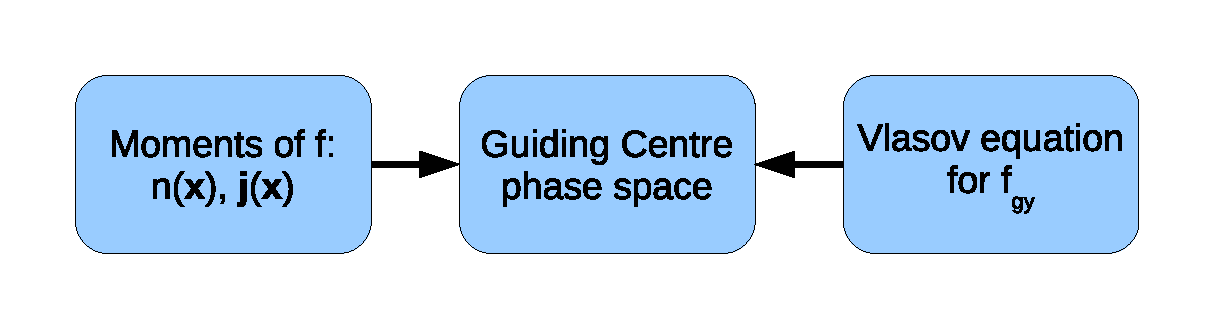
\includegraphics[scale=0.5]{maxwell-transform.eps}
 \end{center}
 \caption{Idea of gyrokinetic Maxwell's equations: The density and current of particles as well as the gyro-centre distribution function are expressed in guiding centre phase space.}
 \label{fig:maxwell-transform}
\end{figure}

As a first step, the particle densities and currents of one species are expressed with the guiding-centre distribution function:
\begin{eqnarray}
	n(\mathbf{x}) &=& \int f(\mathbf{x},\mathbf{v}) \mathrm{d} \mathbf{v} = \frac{B_0}{m} \int \delta(\mathbf{X}+\mathbf{r}-\mathbf{x}) f_{\st{gc}} \mathrm{d}\mathbf{X} \mathrm{d}v_{\parallel} \mathrm{d} \theta \mathrm{d}\mu \label{eq:gc_n} \\
	j_{\parallel} &=& Z e \int v_{\parallel} f(\mathbf{x},\mathbf{v}) \mathrm{d} \mathbf{v}  = \frac{Z e B_0}{m} \int \delta(\mathbf{X}+\mathbf{r}-\mathbf{x}) v_{\parallel} f_{\st{gc}} \mathrm{d}\mathbf{X} \mathrm{d}v_{\parallel} \mathrm{d} \theta \mathrm{d}\mu \label{eq:gc_j_par}\\
	\mathbf{j}_{\perp} &=& Z e \int \vec{v}_{\st{L}} f(\mathbf{x},\mathbf{v}) \mathrm{d} \mathbf{v} = \frac{Z e B_0}{m} \int \delta(\mathbf{X}+\mathbf{r}-\mathbf{x}) \vec{v}_{\st{L}} f_{\st{gc}} \mathrm{d}\mathbf{X} \mathrm{d}v_{\parallel} \mathrm{d} \theta \mathrm{d}\mu \label{eq:gc_j_perp}
\end{eqnarray}
where $\vec{r}$ is the vector pointing from the centre of the Larmor orbit to the particle's position. The $\frac{B_0}{m}$ factor is the Jacobian. Formally, the delta function appears since the change of coordinates affects the whole phase space while the integral goes only over the velocity subspace. It guarantees that the spatial region taken into account in the integral remains unchanged during the coordinate transformation. Physically it expresses that all the particles that have a Larmor orbit crossing a given point $\vec{x}$ in real space contribute to the particle density there (see figure \ref{fig:density-gc}). 

\begin{figure}
 \begin{center}
	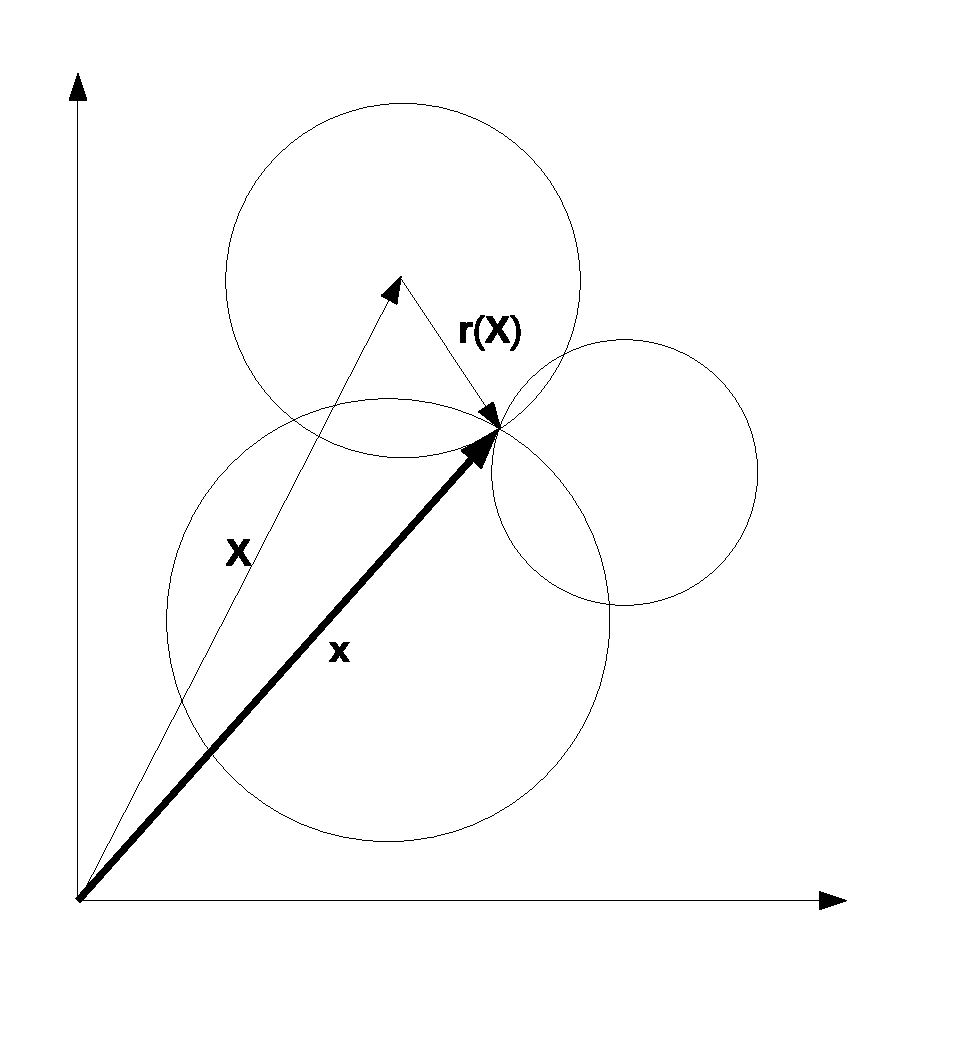
\includegraphics[scale=0.3]{density-gc.eps}
 \end{center}
 \caption{The connection between the density of particles and density of guiding-centres.}
 \label{fig:density-gc}
\end{figure}

The second step is to express the guiding-centre distribution function with the gyro-centre one and write it into equations \ref{eq:gc_n}-\ref{eq:gc_j_perp}. Since the distribution function is a regular function (or zero-form) on the manifold, it is transformed by the pull-back operator:
\begin{equation}
	f_{\st{gc}} = \Phi^* f_{\st{gy}} = \mathrm{e}^{\varepsilon \mathcal{L}_{G_1}} f_{\st{gy}} \approx \left( 1 + \varepsilon \mathcal{L}_{G_1} \right) f_{\st{gy}} = f_{\st{gy}} + G_1^{\nu} \frac{\partial f_{\st{gy}}}{\partial Z^{\nu}}. \label{eq:pullback}
\end{equation}
Substituting the components of the generator vector field derived in section \ref{sec:gyro_derive}, the expressions that connect the gyro-centre and guiding-centre distribution function are directly obtained. The delta-f approximation is applied once again and the equilibrium part of the gyro-centre distribution function $f_{\st{gy}}$ is assumed Maxwellian (equation \ref{eq:maxwellian}). Since the generator functions are already first order in $\rho_*$, in the second part of equation \ref{eq:pullback} only the equilibrium distribution function $F_{\st{M}}$ must be taken into account. Also, as $\nabla F_{\st{M}}$ only contains first order terms in $\rho_*$ the term $G_1^{\mathbf{X}} \cdot \nabla F_{\st{M}}$ can be dropped. The resulting transformation formula is
\begin{eqnarray}
 	G_1^{\mu} \frac{\partial F_{\st{M}}}{\partial \mu} &=& \frac{1}{B_0} \left( Z e \widetilde{\Phi}_1 - Z e v_{\parallel} \widetilde{A}_{1 \parallel} - Z e \left( \widetilde{\mathbf{A}_1 \cdot \vec{v}_{\st{L}}} \right) + Z e v_{\st{L}} \left| \mathbf{A}_{1 \perp}\right| \right) \frac{\partial F_{\st{M}}}{\partial \mu} \nonumber \\
	&=& \frac{1}{B_0} \left( Z e \widetilde{\Phi}_1 - Z e v_{\parallel} \widetilde{A}_{1 \parallel} - Z e \langle \mathbf{A}_1 \cdot \vec{v}_{\st{L}} \rangle \right) \frac{\partial F_{\st{M}}}{\partial \mu} \nonumber \\
	&=& -\frac{1}{T} \left( Z e \widetilde{\Phi}_1 - Z e v_{\parallel} \widetilde{A}_{1 \parallel} + \mu \bar{B}_{1 \parallel} \right) F_{\st{M}} \nonumber \\
	\noalign{\vskip 0.5 truecm}
	G_1^{v_{\parallel}} \frac{\partial F_{\st{M}}}{\partial v_{\parallel}} &=& - Z e \frac{v_{\parallel}}{T} \widetilde{A}_{1 \parallel} F_{\st{M}} \nonumber \\
	\noalign{\vskip 0.5 truecm}
	f_{\st{gc}} &=& f_{\st{gy}} + G_1^{\mu} \frac{\partial F_{\st{M}}}{\partial \mu} + G_1^{v_{\parallel}} \frac{\partial F_{\st{M}}}{\partial v_{\parallel}} = f_{\st{gy}} - \frac{F_{\st{M}}}{T} \left( Z e \widetilde{\Phi}_1 - \mu \bar{B}_{1 \parallel} \right).
	\label{eq:f_gy_to_gc}
\end{eqnarray}
The two correction terms appearing in equation \ref{eq:f_gy_to_gc} containing the fluctuations of the electro-magnetic fields are the results of the pull-back transformation from the gyro-centre to the guiding centre phase space. Physically, they describe the polarization and magnetization effects of the fluctuations on the gyro-orbit \cite{brizard}. 

%-----------------------------------------------------------------------
\subsubsection{Normalization} \label{sec:normalization}
The field equations derived in the following sections will be normalized as detailed in \cite{gkw}. The definition of the normalized quantities is reiterated here for the sake of completeness. A reference mass $m_{\st{ref}}$, density $n_{\st{ref}}$, temperature $T_{\st{ref}}$, magnetic field $B_{\st{ref}}$ and major radius $R_{\st{ref}}$ is chosen. These are then used to define the reference thermal velocity $T_{\st{ref}} = \frac{1}{2} m_{\st{ref}} v_{\st{th,ref}}^2$ and reference thermal Larmor radius $\rho_{\st{ref}} = \frac{m_{\st{ref}} v_{\st{th,ref}}}{e B_{\st{ref}}}$. The normalized major radius and equilibrium magnetic field are simply $R = R_{\st{ref}} R_{st{N}}$ and $B = B_{\st{ref}} B_{\st{N}}$. For convenience, the small parameter $\rho_*$ is redefined with the reference values as $\rho_* = \frac{\rho_{\st{ref}}}{R_{\st{ref}}}$. The reference quantities are used to define the dimensionless relative quantities
\begin{equation}
m_{\st{R}} = \frac{m}{m_{\st{ref}}} \qquad n_{\st{R}} = \frac{n}{n_{\st{ref}}} \qquad T_{\st{R,sp}} = \frac{T}{T_{\st{ref}}} \qquad v_{\st{R}} = \frac{v_{\st{th}}}{v_{\st{th,ref}}}.
\end{equation}
The fluctuating fields are normalized as
\begin{equation}
\Phi_1 = \rho_* \frac{T_{\st{ref}}}{e} \Phi_{1 \st{N}} \qquad A_{1 \parallel} = B_{\st{ref}} R_{\st{ref}} \rho_*^2 A_{1 \parallel \st{N}} \qquad B_{1 \parallel} = \rho_* B_{\st{ref}} B_{1 \parallel \st{N}}.
\end{equation}
The time and the angular rotation frequency are normalized using the reference thermal velocity as
\begin{equation}
t = \frac{R_{\st{ref}}}{v_{\st{th,ref}}} t_{\st{N}} \qquad \Omega = \frac{v_{\st{th,ref}}}{R_{\st{ref}}} \Omega_{\st{N}}
\end{equation}
whereas the velocity space coordinates and the distribution functions are normalized with the thermal velocity to maintain their species dependence:
\begin{equation}
v_{\parallel} = v_{\st{th}} v_{\parallel \st{N}} \qquad \mu = \frac{m v_{\st{th}}^2}{e B_{\st{ref}}} \qquad \delta f = \rho_* \frac{n}{v_{\st{ref}}^3} \delta f_{\st{N}} \qquad F_{\st{M}} = \frac{n}{v_{\st{ref}}^3} F_{\st{M,N}}.
\end{equation}
Finally, the parallel and perpendicular gradients of the equilibrium and the wavenumber of the fluctuations are normalized, respectively, as
\begin{equation}
\nabla_{\perp} = \frac{1}{R_{\st{ref}}} \nabla_{\perp \st{N}} \qquad \nabla_{\parallel} = \frac{1}{R_{\st{ref}}} \nabla_{\parallel \st{N}} \qquad k = \frac{k_{\st{N}}}{\rho_*}.
\end{equation}

%-----------------------------------------------------------------------
\subsubsection{Gyrokinetic Poisson equation}
The derivation of the gyrokinetic Maxwell-equations is now straightforward: the distribution function transformed from gyro-centre to guiding-centre phase space by equation \ref{eq:f_gy_to_gc} has to be substituted to the guiding-centre particle density and current equations \ref{eq:gc_n}-\ref{eq:gc_j_perp}. Equation \ref{eq:gc_n} takes the form
\begin{eqnarray*}
	n(\vec{x}) &=& \frac{B_0}{m} \int \delta(\vec{X}+\vec{r}-\vec{x}) \left( f_{\st{gy}}(\vec{X}) - \frac{F_{\st{M}}}{T} \left( Z e \widetilde{\Phi}_1(\vec{X}+\vec{r}) - \bar{B}_{1 \parallel}(\vec{X}) \right)\right) \mathrm{d}\mathbf{X} \mathrm{d}v_{\parallel} \mathrm{d} \theta \mathrm{d}\mu \\
	&=& \bar{n}(\vec{x}) - \frac{B_0}{m} \int \delta(\vec{X}+\vec{r}-\vec{x}) \left( Z e \widetilde{\Phi}_1(\vec{X}+\vec{r}) - \mu \bar{B}_{1 \parallel}(\vec{X}) \right) \frac{F_{\st{M}}}{T} \mathrm{d}\mathbf{X} \mathrm{d}v_{\parallel} \mathrm{d} \theta \mathrm{d}\mu
\end{eqnarray*}
where the density of gyro-centres $\bar{n}$ has been introduced. Note that the distribution functions $f_{\st{gy}}$ depends on $\vec{X}$ as well as the velocity coordinates $v_{\parallel}$, $\mu$ and $\theta$. Here, however, only the spatial dependence is indicated for the gyroaveraging. Writing the oscillating part of the perturbed potential as $\widetilde{\Phi}_1(\vec{X}+\vec{r}) = \Phi_1(\vec{X}+\vec{r}) - \bar{\Phi}_1(\vec{X})$ and integrating the $\Phi_1(\vec{X}+\vec{r})$ term yields
\begin{eqnarray*}
	n(\vec{x}) &=& \bar{n}(\vec{x}) - \frac{ Z e \Phi_1(\vec{x})}{T} n_0(\vec{x}) \\
	&& + \frac{B_0}{m} \int \delta(\vec{X}+\vec{r}-\vec{x}) \left( Z e \bar{\Phi}_1(\vec{X}) + \mu \bar{B}_{1 \parallel}(\vec{X}) \right) \frac{F_{\st{M}}}{T} \mathrm{d}\mathbf{X} \mathrm{d}v_{\parallel} \mathrm{d} \theta \mathrm{d}\mu
\end{eqnarray*}
where $n_0$ is the equilibrium particle density. The factor $\frac{F_{\st{M}}}{T}$ changes on the equilibrium length scale. Therefore, its weak spatial dependence has been neglected in the previous step compared to the fast variation of the fluctuating $\Phi_1$. 
The integral over $\vec{X}$ together with the delta function changes the arguments of the fields to $\vec{x}-\vec{r}$. After integrating over $\theta$ this results
\begin{eqnarray*}
	n(\vec{x}) &=& \bar{n}(\vec{x}) - \frac{Z e \Phi_1(\vec{x})}{T} n_0(\vec{x}) \\
	&& + \frac{2 \pi B_0}{m} \int J_0(\lambda) \left( Z e \bar{\Phi}_1(\vec{x}) + \mu \bar{B}_{1 \parallel}(\vec{x}) \right) \frac{F_{\st{M}}}{T} \mathrm{d}v_{\parallel} \mathrm{d}\mu
\end{eqnarray*}
where $\lambda^2 = - \rho^2 \nabla_{\perp}^2$. Performing the $v_{\parallel}$ integral is straightforward as it is only the Maxwellian that depends on it: 
\begin{eqnarray*}
	F_{\st{M}} &=& F_{\st{M}}(\mu) \mathrm{e}^{-\frac{m (v_{\parallel} - u_{\parallel})^2}{2 T}} \st{e}^{-\frac{\mathcal{E}}{T}} \\
	n(\vec{x}) &=& \bar{n}(\vec{x}) - \frac{Z e \Phi_1(\vec{x})}{T} n_0(\vec{x}) \\
	&& + \frac{B_0}{\sqrt{T}} \left( \frac{2 \pi}{m} \right)^{\frac{3}{2}} \st{e}^{\frac{-\mathcal{E}}{T}} \int F_{\st{M}}(\mu) J_0(\lambda) \left( Z e \bar{\Phi}_1(\vec{x}) + \mu \bar{B}_{1 \parallel}(\vec{x}) \right) \mathrm{d}\mu.
\end{eqnarray*}
In order to evaluate the integrals of the Bessel functions, let us introduce the new variable $x = \frac{\mu B}{T}$, leading to $\lambda^2 = 2 x b$, $b = -\rho_{\st{th}}^2 \nabla^2_{\perp}$, where $\rho_{\st{th}}$ is the thermal Larmor radius. The two remaining integrals are of the form
\[ \int \limits_0^{\infty} J_0^2(\sqrt{2bx}) \mathrm{e}^{-x} \mathrm{d}x \qquad \int \limits_0^{\infty} J_0(\sqrt{2bx}) \hat{J}_1(\sqrt{2bx}) \sqrt{x} \mathrm{e}^{-x} \mathrm{d}x. \]
For the details of evaluating these integrals see appendix \ref{app:bessel_integral}. The results are
\[\mathrm{e}^{-b} I_0(b) \qquad \mathrm{e}^{-b} \left( I_0(b) - I_1(b) \right) ,\]
respectively, where $I_n$ is the n-th order modified Bessel function of the first kind. Using the notation $\Gamma_n(b) = I_n(b) \mathrm{e}^{-b}$, the expression for the particle density can be written as
\[n(\vec{x}) = \bar{n}(\vec{x}) - \frac{Z e \Phi_1(\vec{x})}{T} n_0(\vec{x}) + n_0 \st{e}^{\frac{-\mathcal{E}}{T}} \left( \Gamma_0(b) \frac{Z e \Phi_1(\vec{x})}{T} + (\Gamma_0(b) - \Gamma_1(b)) \frac{B_{1 \parallel}(\vec{x})}{B_0} \right). \]
The quasineutrality equation $\sum_{\st{sp}} Z_{\st{sp}} e n_{\st{sp}} = 0$ gives
\begin{eqnarray}
	&& \sum_{\st{sp}} Z_{\st{sp}} e \left( 1 - \st{e}^{\frac{-\mathcal{E}_{\st{sp}}}{T_{\st{sp}}}} \Gamma_0(b_{\st{sp}}) \right) \frac{Z_{\st{sp}}e \Phi_1(\vec{x}) n_{0,\st{sp}}}{T_{\st{sp}}} =  \nonumber \\
	&& \hspace{1cm} \sum_{\st{sp}} Z_{\st{sp}} e \left( \bar{n}_{\st{sp}} + \st{e}^{\frac{-\mathcal{E}_{\st{sp}}}{T_{\st{sp}}}} (\Gamma_0(b_{\st{sp}}) - \Gamma_1(b_{\st{sp}})) \frac{B_{1 \parallel}(\vec{x}) n_{0,\st{sp}}}{B_0} \right).
	\label{eq:neutrality}
\end{eqnarray}

In order to bring this equation to the form implemented in GKW, the modified distribution function $g$ has to be applied. When substituting equation \ref{eq:g} into the definition of the gyro-centre density, it can be seen that the second term provides zero contribution since it contains the product of $F_{\st{M}}$, which is symmetric in $v_{\parallel}$, with $v_{\parallel}$, which is antisymmetric:
\begin{eqnarray*}
	\bar{n}(\vec{x}) &=& \frac{B_0}{m} \int \delta(\vec{X}+\vec{r}-\vec{x}) f_{\st{gy}}(\vec{X}) \mathrm{d} \vec{X} \mathrm{d} v_{\parallel} \mathrm{d} \mu \mathrm{d} \theta \\
	&=& \frac{2 \pi B_0}{m} \int J_0(\lambda) \left( g(\vec{x}) - \frac{F_{\st{M}}}{T} v_{\parallel} Z e \bar{A}_{1 \parallel}\right) \mathrm{d}v_{\parallel} \mathrm{d} \mu = \frac{2 \pi B_0}{m} \int J_0(\lambda) g(\vec{x}) \mathrm{d}v_{\parallel} \mathrm{d} \mu.
	\label{eq:density_gkw_nonorm}
\end{eqnarray*}

After Fourier-transforming and applying the normalizing expressions of section \ref{sec:normalization}, the gyrokinetic Poisson equation finally takes the form
\begin{eqnarray}
	\hspace{-5mm}
	&& \sum_{\st{sp}} Z_{\st{sp}} n_{\st{R,sp}} \left[ 2 \pi B_{\st{N}} \int J_0(k_{\perp} \rho_{\st{sp}}) \hat{g}_{\st{N,sp}} \mathrm{d} v_{\parallel N} \mathrm{d} \mu_{\st{N}} + \right. \nonumber \\ 
	\hspace{-5mm}
	&& \left. \frac{Z_{\st{sp}}}{T_{\st{R,sp}}} \hat{\Phi}_{1 \st{N}} \left( \st{e}^{\frac{-\mathcal{E}_{\st{N,sp}}}{T_{\st{R,sp}}}} \Gamma_0(b_{\st{sp}}) - 1 \right) + \frac{\hat{B}_{1 \parallel \st{N}}}{B_{\st{N}}} \st{e}^{\frac{-\mathcal{E}_{\st{N,sp}}}{T_{\st{R,sp}}}} (\Gamma_0(b_{\st{sp}}) - \Gamma_1(b_{\st{sp}})) \right] = 0.
	\label{eq:poisson}
\end{eqnarray}
Since the equation does not contain spatial derivatives of the fields and the distribution function, and they are linear in every term, the Fourier transform simply results in the Fourier components $\hat{g}_{\st{N,sp}}(\vec{k})$, $\hat{\Phi}_{1 \st{N}}(\vec{k})$ and $\hat{B}_{1 \parallel \st{N}}(\vec{k})$.

%-----------------------------------------------------------------------
\subsubsection{Equation for $A_{1 \parallel}$}
The method to calculate the equation of the parallel perturbation of the vector potential is analogous to that used for the Poisson-equation.
The starting point is the parallel component of Amp\`ere's law. It is first transformed into guiding-centre coordinates, then the guiding-centre distribution function is expressed with the pull-back of its gyro-centre counterpart. 

The parallel component of Amp\`ere's law using Coulomb gauge $\nabla \cdot \mathbf{A}_1 = 0$ can be written as
\begin{equation} 
 \nabla^2 \mathbf{A}_{1 \parallel} = \mu_0 \mathbf{j}_{1 \parallel}. 
 \label{eq:ampere}
\end{equation}
The parallel perturbation of the current density is expressed with equation \ref{eq:gc_j_par}. After applying equation \ref{eq:f_gy_to_gc} it takes the form
\begin{eqnarray*}
	j_{1 \parallel} &=& \frac{Z e B_0}{m} \int v_{\parallel} \delta(\vec{X}+\vec{r}-\vec{x}) \left[ f_{\st{gy}}(\vec{X}) - \frac{F_{\st{M}}}{T} \left( Z e \widetilde{\Phi}_1(\vec{X} + \vec{r}) - \mu \bar{B}_{1 \parallel}(\vec{X}) \right) \right] \mathrm{d} \vec{X} \mathrm{d} v_{\parallel} \mathrm{d} \mu \mathrm{d} \theta \\
	&=& \frac{Z e B_0}{m} \int v_{\parallel} \delta(\vec{X}+\vec{r}-\vec{x}) f_{\st{gy}}(\vec{X}) \mathrm{d} \vec{X} \mathrm{d} v_{\parallel} \mathrm{d} \mu \mathrm{d} \theta - \frac{Z e B_0}{m} \underbrace{\int v_{\parallel} F_{\st{M}}(v_{\parallel}) \mathrm{d} v_{\parallel}}_{0} \int (\dots) \mathrm{d} \vec{X} \mathrm{d} \mu \mathrm{d} \theta \\
	&=& \frac{2 \pi Z e B_0}{m} \int v_{\parallel} J_0(\lambda) f_{\st{gy}}(\vec{x}) \mathrm{d} v_{\parallel} \mathrm{d} \mu.
\end{eqnarray*}
Substituting equation \ref{eq:g} gives
\begin{eqnarray*}
	j_{1 \parallel} &=& \frac{2 \pi Z e B_0}{m} \int v_{\parallel} J_0(\lambda) g \mathrm{d} v_{\parallel} \mathrm{d} \mu - \frac{2 \pi Z e B_0}{m} \int v_{\parallel}^2 J_0(\lambda) \frac{F_{\st{M}}}{T} Z e \bar{A}_{1 \parallel} \mathrm{d} v_{\parallel} \mathrm{d} \mu.
\end{eqnarray*}
In the second term the integral over $v_{\parallel}$ can be performed by parts leading to
\[-\frac{ 2 Z^2 e^2 B_0 n_0}{ m^2 v_{\st{th}}^{2}} A_{1 \parallel} \st{e}^{\frac{-\mathcal{E}}{T}} \underbrace{\int J_0^2(\lambda) \mathrm{e}^{-\frac{\mu B_0}{T}} \mathrm{d} \mu}_{\frac{T}{B_0} \Gamma_0(b)},\]
and so the total expression for $j_{1 \parallel}$ becomes
\[j_{1 \parallel} = \frac{2 \pi B_0 Z e}{m} \int v_{\parallel} J_0(\lambda) g \mathrm{d} v_{\parallel} \mathrm{d} \mu - \frac{Z^2 e^2 n_0}{m} \st{e}^{\frac{-\mathcal{E}}{T}} \Gamma_0(b) A_{1 \parallel}. \]
Summing the above expression over the species, substituting into Amp\`ere's law, Fourier transforming and applying the normalization equations yield
\begin{eqnarray}
	&& \left[ k_{\perp N}^2 + \beta_{\st{ref}} \sum_{\st{sp}} \frac{Z_{\st{sp}}^2 n_{\st{R,sp}}}{m_{\st{R,sp}}} \st{e}^{\frac{-\mathcal{E}_{\st{N,sp}}}{T_{\st{R,sp}}}} \Gamma_0(b_{\st{sp}}) \right] \hat{A}_{1 \parallel \st{N}} = \nonumber \\
	&& 2 \pi B_{N} \beta_{\st{ref}} \sum_{\st{sp}} Z_{\st{sp}} n_{\st{R,sp}} v_{\st{R,sp}} \int v_{\parallel N} J_0(k_{\perp} \rho_{\st{sp}}) \hat{g}_{\st{N,sp}} \mathrm{d} v_{\parallel N} \mathrm{d} \mu_{N}
	\label{eq:apar}
\end{eqnarray}
where the reference plasma beta has been defined as
\begin{equation}
	\beta_{\st{ref}} = \frac{2 \mu_0 n_{\st{ref}} T_{\st{ref}}}{B_{\st{ref}}^2}.
	\label{eq:beta}
\end{equation}


%-----------------------------------------------------------------------
\subsubsection{Equation for $B_{1 \parallel}$}
The perpendicular component of Amp\`ere's law can be written as
\[ (\nabla \times \mathbf{B}_1)_{\perp} = \left( \begin{array}{c} \partial_y B_{1 \parallel} - \partial_z B_{1 y} \\ \partial_z B_{1x} - \partial_x B_{1 \parallel} \end{array} \right) = \mu_0 \mathbf{j}_{1 \perp} \]
where $z$ is the direction of the equilibrium magnetic field. The parallel gradients of the perturbed quantities can be neglected since they are one order smaller than perpendicular ones, giving
\begin{equation*}
	\left( \begin{array}{c} \partial_y B_{1 \parallel} \\ - \partial_x B_{1 \parallel} \end{array} \right) = \nabla_{\perp} B_{1 \parallel} \times \mathbf{b} = \mu_0 \mathbf{j}_{1 \perp}.
\end{equation*}
Taking the cross-product of the above equation with $\vec{b}$ from the left gives
\[ \mu_0 \vec{b} \times \vec{j}_{1 \perp} = \vec{b} \times \nabla_{\perp} B_{1 \parallel} \times \vec{b} = \nabla_{\perp} B_{1 \parallel}. \]
Using equation \ref{eq:gc_j_perp}, assuming zero equilibrium current $\vec{j}_0 = 0$, summing over species and dotting with $\vec{k}_{\perp}$ leads to
\begin{eqnarray*}
	\vec{k}_{\perp} \cdot \nabla_{\perp} B_{1 \parallel} &=& \mu_0 B_0 e \sum_{\st{sp}} \frac{Z_{\st{sp}}}{m_{\st{sp}}} \int \delta(\vec{X}+\vec{r}-\vec{x}) \underbrace{\vec{k}_{\perp} \cdot \vec{b} \times \vec{v}_{\st{L}}}_{\vec{v}_{\st{L}} \cdot (\vec{k}_{\perp} \times \vec{b})} \\ 
	&& \left( f_{\st{gy,sp}} - \left( Z_{\st{sp}} e \widetilde{\Phi}_{1} - \mu \bar{B}_{1 \parallel} \right) \frac{F_{\st{M}}}{T_{\st{sp}}} \right) \mathrm{d} \vec{X} \mathrm{d} v_{\parallel} \mathrm{d} \mu \mathrm{d} \theta \\
	&=& \mu_0 B_0 e \sum_{\st{sp}} \frac{Z_{\st{sp}}}{m_{\st{sp}}} \left[ \int \vec{v}_{\st{L}} \cdot (\vec{k}_{\perp} \times \vec{b}(\vec{x})) f_{\st{gy,sp}}(\vec{x}-\vec{r}) \mathrm{d} v_{\parallel} \mathrm{d} \mu \mathrm{d} \theta \right. \\ 
	&& \left. + \int \vec{v}_{\st{L}} \cdot (\vec{k}_{\perp} \times \vec{b}(\vec{x})) \frac{F_{\st{M}}}{T_{\st{sp}}}\left( Z_{\st{sp}} e \bar{\Phi}_1(\vec{x}-\vec{r}) + \mu \bar{B}_{1 \parallel}(\vec{x}-\vec{r}) \right)  \mathrm{d} v_{\parallel} \mathrm{d} \mu \mathrm{d} \theta \right].
\end{eqnarray*}
Performing the $\theta$-integral gives (for details see \cite{dannert}, Appendix C)
\begin{eqnarray*}
	\vec{k}_{\perp} \cdot \nabla_{\perp} B_{1 \parallel} &=& - 2 \pi \mu_0 B_0 e \sum_{\st{sp}} \frac{Z_{\st{sp}}}{|Z_{\st{sp}}|} \frac{Z_{\st{sp}}}{m_{\st{sp}}} \left[ v_{\st{L}} \int \frac{\mathrm{d}^3 k}{(2 \pi)^3} \left( i k_{\perp}^2 (\vec{k}_{\perp} \times \vec{b} \cdot \vec{e}_1 \hat{f}_{\st{gy,sp}}) - \right. \right. \\ 
	&& \left. i k_{\perp}^1 (\vec{k}_{\perp} \times \vec{b} \cdot \vec{e}_2 \hat{f}_{\st{gy,sp}}) \right) \frac{\rho_{\st{sp}}}{2} \hat{J}_1(k_{\perp} \rho_{\st{sp}}) \mathrm{e}^{i \vec{k} \cdot \vec{r}} \mathrm{d} v_{\parallel} \mathrm{d} \mu + \\
	&& v_{\st{L}} \int \frac{\mathrm{d}^3 k}{(2 \pi)^3} i k_{\perp}^2 \left( \vec{k}_{\perp} \times \vec{b} \cdot \vec{e}_1 \frac{F_{\st{M}}}{T_{\st{sp}}} \left( Z_{\st{sp}} e \hat{\bar{\Phi}}_1 + \mu \hat{\bar{B}}_{1 \parallel} \right) \right) - \\ 
	&& \left. i k_{\perp}^1 \left( \vec{k}_{\perp} \times \vec{b} \cdot \vec{e}_2 \frac{F_{\st{M}}}{T_{\st{sp}}} \left( Z_{\st{sp}} e \hat{\bar{\Phi}}_1 + \mu \hat{\bar{B}}_{1 \parallel} \right) \right) \frac{\rho_{\st{sp}}}{2} \hat{J}_1(k_{\perp} \rho_{\st{sp}}) \mathrm{e}^{i \vec{k} \cdot \vec{r}} \mathrm{d} v_{\parallel} \mathrm{d} \mu \right].
\end{eqnarray*}
It can be easily shown that $\vec{k}_{\perp} \times \vec{b} \cdot \vec{e}_1 = k_{\perp}^2$ and $\vec{k}_{\perp} \times \vec{b} \cdot \vec{e}_2 = -k_{\perp}^1$, where the upper indices represent contravariant components. Fourier transforming both sides, dividing by the perpendicular wavenumber and transforming back to real space results
\begin{eqnarray*}
	i k_{\perp}^2 \hat{B}_{1 \parallel} &=& - 2 \pi B_0 e \mu_0 \sum_{\st{sp}} \frac{Z_{\st{sp}}}{|Z_{\st{sp}}|} \frac{Z_{\st{sp}}}{m_{\st{sp}}} \left[ v_{\st{L}} \int i k_{\perp}^2 \hat{f}_{\st{gy,sp}} \frac{\rho_{\st{sp}}}{2} \hat{J}_1(k_{\perp} \rho_{\st{sp}}) \mathrm{d} v_{\parallel} \mathrm{d} \mu \right. + \\ 
	&& \left. v_{\st{L}} \int i k_{\perp}^2 \left( Z_{\st{sp}} e \hat{\bar{\Phi}}_1 + \mu \hat{\bar{B}}_{1 \parallel} \right) \frac{F_{\st{M}}}{T_{\st{sp}}} \frac{\rho_{\st{sp}}}{2} \hat{J}_1(k_{\perp} \rho_{\st{sp}}) \mathrm{d} v_{\parallel} \mathrm{d} \mu \right] \\
	B_{1 \parallel} &=& - 2 \pi B_0 \mu_0 \sum_{\st{sp}} \frac{Z_{\st{sp}}}{|Z_{\st{sp}}|} \frac{1}{m_{\st{sp}}} \left[ \int \mu \frac{Z_{\st{sp}}}{|Z_{\st{sp}}|} \hat{J}_1(\lambda_{\st{sp}}) f_{\st{gy,sp}} \mathrm{d} v_{\parallel} \mathrm{d} \mu \right. \\
	&& \left. + \int \mu \left( Z_{\st{sp}} e J_0(\lambda_{\st{sp}}) \Phi_1 + \mu \hat{J}_1(\lambda_{\st{sp}}) B_{1 \parallel} \right) \frac{F_{\st{M}}}{T_{\st{sp}}} \frac{Z_{\st{sp}}}{|Z_{\st{sp}}|} \hat{J}_{1}(\lambda_{\st{sp}}) \mathrm{d} v_{\parallel} \mathrm{d} \mu \right].
\end{eqnarray*}
Here the upper index in $k_{\perp}^2$ means second power. The integral over $v_{\parallel}$ is elementary as again it only appears in the Maxwellian. Using equation \ref{eq:g} and evaluating the integrals over $\mu$ according to equations \ref{eq:bessel_integral_bpar} in appendix \ref{app:bessel_integral} one obtains
\begin{eqnarray*}
B_{1 \parallel} &=& - \sum_{\st{sp}} \frac{2 \mu_0 T_{\st{sp}} n_{0,\st{sp}}}{B_0} \left[ \frac{\pi B_0^2}{m_{\st{sp}} n_{0,\st{sp}} T_{\st{sp}}} \int \mu \hat{J}_1(\lambda_{\st{sp}}) g_{\st{sp}} \mathrm{d}v_{\parallel} \mathrm{d} \mu + \right. \nonumber \\
&& \left. \st{e}^{\frac{-\mathcal{E}}{T_{\st{sp}}}} (\Gamma_0(b_{\st{sp}}) - \Gamma_1(b_{\st{sp}})) \left( \frac{Z_{\st{sp}} e \Phi_1}{2 T_{\st{sp}}} + \frac{B_{1 \parallel}}{B_0} \right) \right].
\end{eqnarray*}
Normalization and rearrangement of the terms after writing the fields in Fourier-space yield
\begin{eqnarray}
	&& \left[ 1 + \sum_{\st{sp}} \beta_{\st{sp}} \st{e}^{\frac{-\mathcal{E}_{\st{N,sp}}}{T_{\st{R,sp}}}} \left( \Gamma_0(b_{\st{sp}}) - \Gamma_1(b_{\st{sp}}) \right) \right] \hat{B}_{1 \parallel \st{N}} = \nonumber \\
	&& \hspace{2cm} - \sum_{\st{sp}} \beta_{\st{sp}} \left[ 2 \pi B_{\st{N}}^3 \int \mu_{N} \hat{J}_1(k_{\perp} \rho_{\st{sp}}) \hat{g}_{\st{N,sp}} \mathrm{d}v_{\parallel N} \mathrm{d} \mu_{\st{N}} \right. + \nonumber \\ 
	&& \hspace{2cm} \left. \st{e}^{\frac{-\mathcal{E}_{\st{N,sp}}}{T_{\st{R,sp}}}} \left( \Gamma_0(b_{\st{sp}}) - \Gamma_1(b_{\st{sp}}) \right) \frac{Z_{\st{sp}} B_{\st{N}}}{2 T_{\st{R,sp}}} \hat{\Phi}_{1 \st{N}} \right].
	\label{eq:bpar1}
\end{eqnarray}
Using the reference instead of the full value of the plasma beta ($\beta = \beta_{\st{ref}} \beta_{\st{R}} = \beta_{\st{ref}} \frac{T_{\st{R,sp}} n_{\st{R,sp}}}{B_{\st{N}}^2}$), the equation for the parallel magnetic perturbation can be finally written as
\begin{eqnarray}
	&& \hspace{-1cm} \left[ 1 + \sum_{\st{sp}} \frac{T_{\st{R,sp}} n_{\st{R,sp}}}{B_{\st{N}}^2} \beta_{\st{ref}} \st{e}^{\frac{-\mathcal{E}_{\st{N,sp}}}{T_{\st{R,sp}}}} \left( \Gamma_0(b_{\st{sp}}) - \Gamma_1(b_{\st{sp}}) \right) \right] \hat{B}_{1 \parallel \st{N}} = \nonumber \\
	&& \hspace{1cm} - \sum_{\st{sp}} \beta_{\st{ref}} \left[ 2 \pi B_{\st{N}} T_{\st{R,sp}} n_{\st{R,sp}} \int \mu_{N} \hat{J}_1(k_{\perp} \rho_{\st{sp}}) \hat{g}_{\st{N,sp}} \mathrm{d}v_{\parallel N} \mathrm{d} \mu_{\st{N}} \right. \nonumber\\
	&& \hspace{1cm} + \left. \st{e}^{\frac{-\mathcal{E}_{\st{N,sp}}}{T_{\st{R,sp}}}} \left( \Gamma_0(b_{\st{sp}}) - \Gamma_1(b_{\st{sp}}) \right) \frac{Z_{\st{sp}} n_{\st{R,sp}}}{2 B_{\st{N}}} \hat{\Phi}_{1 \st{N}} \right].
	\label{eq:bpar}
\end{eqnarray}

It can be seen that both the perpendicular (equation \ref{eq:apar}) and parallel (equation \ref{eq:bpar1}) components of the perturbed magnetic field depend strongly on the plasma $\beta$. Indeed, it has been commonly observed in gyrokinetic simulations that in low $\beta$ plasmas the amplitude of the magnetic perturbations is much lower than that of the fluctuating scalar potential. However, in high $\beta$ plasmas magnetic perturbations strongly impact mode stability and transport by destabilizing kinetic ballooning \cite{jenko_em} and micro-tearing \cite{applegate_mtm} modes.

The correction suggested in equation \ref{eq:bpar1} compared to the calculation by Dannert in \cite{dannert} is the missing $2 b$ factor in the second term on the left hand side, which is the direct consequence of equation \ref{eq:bessel_integral_bpar}. High $\beta$ simulations with GKW using the corrected form of this equation have been successfully benchmarked against an other gyrokinetic code, GS2 \cite{gs2}.



%-----------------------------------------------------------------------
\newpage

\begin{thebibliography}{99}
 \bibitem{dannert} T. Dannert: Gyrokinetische Simulation von Plasmaturbulenz mit gefangenen Teilchen und Elektromagnetischen Effekten (Doctoral Thesis, Technische Universt\"at M\"unchen, 2005)
 \bibitem{gkw} A.G. Peeters et al. (including G. Szepesi), Comput. Phys. Commun. {\bf 180}, 2650 (2009)
 \bibitem{bellan} P.M. Bellan, Fundamentals of Plasma Physics (Cambridge University Press, 2006)
 \bibitem{brizard} A.J. Brizard, T.S. Hahm, Reviews of Modern Physics {\bf 79}, 421 (2007)
 \bibitem{littlejohn_gc} R.G. Littlejohn, Phys. Fluids {\bf 24}, 1730 (1981)
 \bibitem{fecko} M. Fecko Differential Geometry and Lie Groups for Physicists (Cambridge University Press, 2006) 
 \bibitem{littlejohn} R.G. Littlejohn, J. Math. Phys. {\bf 23}, 742 (1982)
 \bibitem{peeters_rotation} A.G. Peeters et al., Phys. Plasmas {\bf 16}, 042310 (2009)
 \bibitem{scott_gotit} B. Scott: Introduction to Gyrokinetic Field Theory (Lecture notes, GOTiT course at IPP Garching, 2008 November)
 \bibitem{Casson2010} F.J. Casson et al. (including G. Szepesi), Phys. Plasmas {\bf 17}, 102305 (2010)
 \bibitem{a_and_s} M. Abramowitz, I.A. Stegun, eds., Handbook of Mathematical Functions with Formulas, Graphs, and Mathematical Tables, (New York: Dover Publications, 1972)
 \bibitem{jenko_em} F. Jenko, W. Dorland, Plasma Phys. Control. Fusion {\bf 43}, A141 (2001)
 \bibitem{applegate_mtm} D J Applegate et al., Plasma Phys. Control. Fusion {\bf 49}, 1113 (2007)
 \bibitem{gs2} M. Kotschenreuther, G. Rewoldt, and M. W. Tang, Comput. Phys. Commun. {\bf 88}, 128 (1995)
\bibitem{g_and_r} I.S Gradshteyn, I.M. Ryzhik: Table of integrals, series, and products (Academic Press, 1965)
 \bibitem{w_and_w} E.T. Whittaker, G.N. Watson, A Course of Modern Analysis (Cambridge University Press, 4th edition, 1927)
\end{thebibliography}



%-----------------------------------------------------------------------
\newpage

\appendix
% \appendixpage

%-----------------------------------------------------------------------
\section{Integrals involving products of Bessel functions} \label{app:bessel_integral}
The following three types of integrals involving products of Bessel functions, exponential and algebraic terms appear in the derivation of the gyrocentre Maxwell's equations:
\begin{eqnarray}
	1. && \int \limits_{0}^{\infty} J_0^2(\lambda) \mathrm{e}^{-\frac{\mu B_0}{T}} \mathrm{d} \mu \\
	2. && \int \limits_{0}^{\infty} \mu J_0(\lambda) \hat{J}_1(\lambda) \mathrm{e}^{-\frac{\mu B_0}{T}} \mathrm{d} \mu \\
	3. && \int \limits_{0}^{\infty} \mu^2 \hat{J}_1^2(\lambda) \mathrm{e}^{-\frac{\mu B_0}{T}} \mathrm{d} \mu
\end{eqnarray}
where $\hat{J}_1(\lambda) = \frac{2}{\lambda} J_1(\lambda)$. In all three cases the new variable $x = \frac{\mu B_0}{T}$ is introduced according to Dannert \cite{dannert}, which also leads to $\lambda = \sqrt{2 x b}$ where $b = - \rho_{th}^2 \nabla_{\perp}^2$. The Jacobian is simply $\frac{T}{B_0}$ and the integrals can be written as
\begin{eqnarray*}
	1. && \frac{T}{B_0} \int \limits_{0}^{\infty} J_0^2(\sqrt{2 x b}) \mathrm{e}^{-x} \mathrm{d} x \\
	2. && \frac{T^2}{B_0^2} \frac{2}{\sqrt{2b}} \int \limits_{0}^{\infty} \sqrt{x} J_0(\sqrt{2 x b}) J_1(\sqrt{2 x b}) \mathrm{e}^{-x} \mathrm{d} x \\
	3. && \frac{T^3}{B_0^3} \frac{2}{b} \int \limits_{0}^{\infty} x J_1^2(\lambda) \mathrm{e}^{-\frac{\mu B_0}{T}} \mathrm{d} x.
\end{eqnarray*}
The first integral can be solved using the formula 6.615 on page 710 of \cite{g_and_r}:
\[\int \limits_0^{\infty} \mathrm{e}^{- \alpha x} J_{\nu}(2 \beta \sqrt{x}) J_{nu}(2 \gamma \sqrt{x}) \mathrm{d} x = \frac{1}{\alpha} I_{\nu}\left( \frac{2 \beta \gamma}{\alpha} \right) \mathrm{e}^{-\frac{\beta^2 + \gamma^2}{\alpha^2}}\]
which immedately gives
\begin{eqnarray*}
	1. && \frac{T}{B_0} \int \limits_{0}^{\infty} J_0^2(\sqrt{2 x b}) \mathrm{e}^{-x} \mathrm{d} x = I_0(b) \mathrm{e}^{-b}.
\end{eqnarray*}
In the two remaining integrals let us use the new variable $y=\sqrt{2 b x}$. The Jacobian is $\frac{y}{b}$ and therefore it leads to
\begin{eqnarray*}
	2. && \frac{T^2}{B_0^2} \frac{2}{\sqrt{2b}} \int \limits_{0}^{\infty} \sqrt{x} J_0(\sqrt{2 x b}) J_1(\sqrt{2 x b}) \mathrm{e}^{-x} \mathrm{d} x = \frac{T^2}{B_0^2} \frac{1}{b^2} \int \limits_{0}^{\infty} y^2 J_0(y) J_1(y) \mathrm{e}^{-h y^2} \mathrm{d}y \\
	3. && \frac{T^3}{B_0^3} \frac{2}{b} \int \limits_{0}^{\infty} x J_1^2(\lambda) \mathrm{e}^{-\frac{\mu B_0}{T}} \mathrm{d} \mu = \frac{T^3}{B_0^3} \frac{1}{b^3} \int \limits_{0}^{\infty} y^3 J_1^2(y) \mathrm{e}^{-h y^2} \mathrm{d} y
\end{eqnarray*}
where $h = \frac{1}{2b}$ was used in the exponentials. 

The second integral (leaving the prefactors for now) can be further written as
\begin{eqnarray*}
	\int \limits_{0}^{\infty} y^2 J_0(y) J_1(y) \mathrm{e}^{-h y^2} \mathrm{d}y &=& \frac{\partial}{\partial h} \left( - \int \limits_0^{\infty} \mathrm{e}^{-hy^2} J_0(y) J_1(y) \right) \mathrm{d} y\\
	&=& \frac{1}{2} \frac{\partial}{\partial h} \left( \int \limits_0^{\infty} \mathrm{e}^{-hy^2} \frac{\mathrm{d}}{\mathrm{d} y} \left(J_0^2(y)\right) \right) \mathrm{d}y \\
	&=& \frac{1}{2} \frac{\partial}{\partial h} \left( \underbrace{\left[ J_0^2(y) \mathrm{e}^{-h y^2} \right]_0^{\infty}}_{1}  + 2 h \int \limits_0^{\infty} J_0^2(y) y \mathrm{e}^{-h y^2} \mathrm{d}y \right)
\end{eqnarray*}
where the relation $\frac{\mathrm{d} J_0(y)}{\mathrm{d} y} = - J_1(y)$ was applied (see \cite{a_and_s}). The integral can be found in \cite{w_and_w} on page 395 and it gives
\begin{equation}
	\int \limits_{0}^{\infty} y J_0^2(y) \mathrm{e}^{-h y^2} \mathrm{d}y = \frac{1}{2h} \mathrm{e}^{-\frac{1}{2h}} I_0\left(\frac{1}{2h}\right).
\end{equation}
Taking the derivative with respect to $h$ and using the identity $\frac{\mathrm{d}I_0(z)}{\mathrm{d} z} = I_1(z)$ results
\begin{eqnarray}
	\int \limits_{0}^{\infty} y^2 J_0(y) J_1(y) \mathrm{e}^{-h y^2} \mathrm{d}y &=& \frac{1}{4h^2} \mathrm{e}^{-\frac{1}{2h}} \left( I_0\left( \frac{1}{2h} \right) - I_1\left( \frac{1}{2h} \right) \right) \nonumber \\
	&=& b^2 \mathrm{e}^{-b} \left( I_0(b) - I_1(b) \right).
	\label{eq:K2}
\end{eqnarray}
And with the prefactors:
\begin{eqnarray}
	2. && \int \limits_{0}^{\infty} \mu J_0(\lambda) \hat{J}_1(\lambda) \mathrm{e}^{-\frac{\mu B_0}{T}} \mathrm{d} \mu = \frac{T^2}{B_0^2} \mathrm{e}^{-b} \left( I_0(b) - I_1(b) \right).
\end{eqnarray}

The third integral (without the prefactors) is integrated by parts first to get
\begin{eqnarray*}
	\int \limits_{0}^{\infty} y^3 J_1^2(y) \mathrm{e}^{-h y^2} \mathrm{d} y &=& -\frac{1}{2 h} \int \limits_{0}^{\infty} (-2 h y) \mathrm{e}^{-h y^2} y^2 J_1(y) \mathrm{d} y \\
	&=& -\frac{1}{2h} \left( \underbrace{\left[ \mathrm{e}^{-h y^2} y^2 J_1^2(y) \right]_0^{\infty}}_{0} - 2 \int \limits_0^{\infty}  \mathrm{e}^{-h y^2} \left( y J_1^2(y) + y^2 J_1(y) \frac{\mathrm{d}J_1(y)}{\mathrm{d}y} \right) \right).
\end{eqnarray*}
Using the relation $\frac{\mathrm{d}J_1(y)}{\mathrm{d}y} = J_0(y) - \frac{1}{y} J_1(y)$ (see \cite{a_and_s}) two of the terms cancel out and the integral simplifies to
\begin{equation}
	\int \limits_{0}^{\infty} y^3 J_1^2(y) \mathrm{e}^{-h y^2} \mathrm{d} y = \frac{1}{h} \int \limits_{0}^{\infty} y^2 J_0(y) J_1(y) \mathrm{e}^{-h y^2} \mathrm{d} y. \nonumber
\end{equation}
Using equation (\ref{eq:K2}) the third integral can be written as
\begin{equation}
	\int \limits_{0}^{\infty} y^3 J_1^2(y) \mathrm{e}^{-h y^2} \mathrm{d} y = 2 b^3 \mathrm{e}^{-b} \left( I_0(b) - I_1(b) \right)
\end{equation}
and with prefactors:
\begin{eqnarray}
	3. && \int \limits_{0}^{\infty} \mu^2 \hat{J}_1^2(\lambda) \mathrm{e}^{-\frac{\mu B_0}{T}} \mathrm{d} \mu = \frac{T^3}{B_0^3} 2 \mathrm{e}^{-b} \left( I_0(b) - I_1(b) \right).
	\label{eq:bessel_integral_bpar}
\end{eqnarray}





\end{document}
